% CVPR 2024 Paper Template; see https://github.com/cvpr-org/author-kit

\documentclass[10pt,twocolumn,letterpaper]{article}

%%%%%%%%% PAPER TYPE  - PLEASE UPDATE FOR FINAL VERSION
\usepackage{cvpr}              % To produce the CAMERA-READY version
% \usepackage[review]{cvpr}      % To produce the REVIEW version
% \usepackage[pagenumbers]{cvpr} % To force page numbers, e.g. for an arXiv version
% Import additional packages in the preamble file, before hyperref
%
% --- inline annotations
%
\usepackage[table,xcdraw,dvipsnames]{xcolor}
% \newcommand{\red}[1]{{\color{red}#1}}
% \newcommand{\todo}[1]{{\color{red}#1}}
% \newcommand{\TODO}[1]{\textbf{\color{red}[TODO: #1]}}
% --- disable by uncommenting  
% \renewcommand{\TODO}[1]{}
% \renewcommand{\todo}[1]{#1}

% \usepackage[caption=false]{subfig}

\usepackage{multirow}
\usepackage[export]{adjustbox}
\usepackage{bbm}
\usepackage{xcolor,amsmath}
%\usepackage{subfigure}
\usepackage[linesnumbered,ruled,vlined]{algorithm2e}
\DontPrintSemicolon

\renewcommand{\KwSty}[1]{\textnormal{\textcolor{blue!90!black}{\ttfamily\bfseries #1}}\unskip}
\renewcommand{\ArgSty}[1]{\textnormal{\ttfamily #1}\unskip}
\SetKwComment{Comment}{\color{green!50!black}// }{}
\renewcommand{\CommentSty}[1]{\textnormal{\ttfamily\color{green!50!black}#1}\unskip}
\newcommand{\assign}{\leftarrow}
\newcommand{\var}{\texttt}
\newcommand{\FuncCall}[2]{\texttt{\bfseries #1(#2)}}
\SetKw{breakloop}{break}
\SetKwProg{Function}{function}{}{}
\renewcommand{\ProgSty}[1]{\texttt{\bfseries #1}}
\newcommand{\bx}{\hat{\boldsymbol{x}}}
\newcommand{\R}{\mathbb{R}}
\newcommand{\ray}{\bold{p}}


\newcommand\lft{\mathopen{}\left}
\newcommand\rgt{\aftergroup\mathclose\aftergroup{\aftergroup}\right}

\newcommand{\GK}[1]{\textcolor{blue}{GK: #1}}
\newcommand{\dv}[1]{\textcolor{red}{DV: #1}}
\newcommand{\am}[1]{\textcolor{orange}{AM: #1}}
\definecolor{darkgreen}{RGB}{0,160,0}
\newcommand{\ph}[1]{\textcolor{darkgreen}{PH: #1}}
\newcommand{\jb}[1]{\textcolor{purple}{JB: #1}}
\newcommand{\yz}[1]{{\color{purple}{\textbf{Yinda: #1}}}}

\newcommand{\scenename}[1]{\textit{#1}}
\newcommand{\figninewidth}{3.1cm}
\newcommand{\figsixwidth}{3.1cm}

% https://tikz.net/zoom/
\newif\ifblackandwhitecycle
\gdef\patternnumber{0}

\makeatletter
\@namedef{ver@everyshi.sty}{}
\makeatother
\usepackage{tikz}
\usepackage{pgfplots}
\usetikzlibrary{spy,calc}

\pgfplotsset{compat=1.16}

\newcommand{\myparagraph}[1]{ \vspace{3pt}  \noindent {\bf #1}\,\,\,}

\newcommand{\acronym}{EVER}
\newcommand{\longname}{Exact Volumetric Ellipsoid Rendering}

\input{sec/zoom}

% It is strongly recommended to use hyperref, especially for the review version.
% hyperref with option pagebackref eases the reviewers' job.
% Please disable hyperref *only* if you encounter grave issues, 
% e.g. with the file validation for the camera-ready version.
%
% If you comment hyperref and then uncomment it, you should delete *.aux before re-running LaTeX.
% (Or just hit 'q' on the first LaTeX run, let it finish, and you should be clear).
\definecolor{cvprblue}{rgb}{0.21,0.49,0.74}
\usepackage[pagebackref,breaklinks,colorlinks,citecolor=cvprblue]{hyperref}

%%%%%%%%% PAPER ID  - PLEASE UPDATE
\def\paperID{12662} % *** Enter the Paper ID here
\def\confName{ICCV}
\def\confYear{2025}

%%%%%%%%% TITLE - PLEASE UPDATE
\title{\acronym{}: \longname{} for Real-time View Synthesis}

\newcommand{\authorbox}[2]{\makebox[0pt][l]{#1$^#2$}\phantom{George Kopanas}}
\newcommand{\aemail}[1]{\makebox[0pt][l]{{\tt\small #1}}\phantom{{\tt\small dfutschik@google.com}}}

\newcommand{\institutes}[0]{$^1$University of California, San Diego \quad $^2$Google \quad $^*$work done while at Google}

%%%%%%%%% AUTHORS - PLEASE UPDATE
\author{
\authorbox{Alexander Mai$^1$}{*}\\
% University of California, San Diego\\
% {\tt\small amai@ucsd.edu}
\aemail{amai@ucsd.edu}
\and
\authorbox{Peter Hedman}{2}\\
% Google\\
\aemail{hedman@google.com}
\and
\authorbox{George Kopanas}{2}\\
% Google\\
\aemail{gkopanas@google.com}
\and
\authorbox{Dor Verbin}{2}\\
% Google\\
\aemail{dorverbin@google.com}
\and
\authorbox{David Futschik}{2}\\
% Google\\
\aemail{dfutschik@google.com}
\and
\authorbox{Qiangeng Xu}{2}\\
% Google\\
\aemail{qiangenx@google.com}
\and
\authorbox{Falko Kuester}{3}\\
% University of California, San Diego\\
\aemail{fkuester@ucsd.edu}
\and
\authorbox{Jonathan T. Barron}{2}\\
% Google\\
\aemail{barron@google.com}
\and
\authorbox{Yinda Zhang}{2}\\
% Google\\
\aemail{yindaz@google.com}
}

\begin{document}

\twocolumn[{%
\renewcommand\twocolumn[1][]{#1}%
\maketitle
\begin{center}
    \centering
%     \begin{tabular}{c@{}c@{}c@{}c@{}c@{}}
% 3DGS & StopThePop & Ours & Ground Truth \\
% \graphimseven{images/comparison_table/3DGS_im7.png} &
% % \graphimseven{images/comparison_table/mcmc_im7.png} &
% \graphimseven{images/comparison_table/stop_im7.png} &
% \graphimseven{images/comparison_table/ours_im7.png} &
% \graphimseven{images/comparison_table/gt_im7.png} \\
%     \end{tabular}
    \includegraphics[width=\textwidth]{figures/Frontpage-Splinetracing2.pdf}

\captionof{figure}{An overview of the quality benefits of our EVER technique. 
Left: On the Zip-NeRF dataset, our model produces the sharpest results ever. 
Middle: Our method is able to blend primitive colors together to reproduce light and shadow better than other 3DGS-based methods.
Right: The way our approach blends colors is physically accurate over any number of primitives, matching the ground truth computed via quadrature.
%Middle: Because our method correctly blends primitive colors according to the physics of volume rendering, it produces fewer ``foggy'' artifacts than splatting. 
%Right: Our method correctly blends primitive colors, which is not possible using a splatting regardless of how primitives are sorted (globally or ray-wise).
}
\label{fig:frontpage}
% Top left: Monastery~\cite{Calidos2023} scene, which requires efficient use of primitives. Top right: "bicycle" scene rendered at 30 FPS. Bottom left: simulated focal length using raytracing. Bottom right: Scene reconstructed from fisheye images.}
\end{center}
}]




% DV abstract, March 6th 2025:
% We present \longname{} (\acronym{}), a method for real-time 3D reconstruction. \acronym{} represents a scene as a large collection of overlapping 3D ellipsoids, each with constant volume density. Unlike prior work on 3D reconstruction, our representation can be efficiently rendered \emph{exactly} without any approximation error which may cause popping or aliasing. We do this by computing the two intersections of every camera ray with the ellipsoids it intersects, and accumulating the derivatives of the densities and colors along the ray. We combine our approach with ray tracing, which enables effects such as defocus blur and fish-eye camera distortion, while still allowing rendering at $\sim\!30$ frames per second at 720p on a single NVIDIA RTX4090. We show that our method is more accurate on the challenging large-scale scenes from the Zip-NeRF dataset, where it achieves state-of-the-art sharpness, even higher than Zip-NeRF.

\begin{abstract}
We present \longname{} (\acronym{}), a method for real-time 3D reconstruction.
\acronym{} accurately blends an unlimited number of overlapping primitives together in 3D space, eliminating the popping artifacts that 3D Gaussian Splatting (3DGS) and other related methods exhibit.
EVER represents a radiance field as a set of constant-density volumetric ellipsoids, which are raytraced by intersecting each primitive twice (once upon ray entrance and another on ray exit) and accumulating the derivatives of the densities and colors along the ray.
Because EVER is built around ray tracing, it also enables effects such as defocus blur and fish-eye camera distortion, while still achieving frame rates of $\sim\!30$ FPS at 720p on an NVIDIA RTX4090. 
We show that our method is more accurate on the challenging large-scale scenes from the Zip-NeRF dataset, where it achieves state of the art SSIM, even higher than Zip-NeRF.
%As such, unlike 3DGS our formulation does not suffer from popping artifacts and view dependent density, but still achieves frame rates of $\sim\!30$ FPS at 720p on an NVIDIA RTX4090. 

%, with none of the blending issues that 3DGS and follow-up work on view-consistent rendering suffer.
% Our method achieves competitive results on the Mip-NeRF dataset and achieves SOTA results on the Zip-NeRF dataset among real-time methods.
% Extensive experiments on various of scenes show that our approach produces renderings with higher fidelity than 3D Gaussian Splatting and comparable quality with SoTA NeRF-based approaches, while achieving framerates of around 30 FPS at 720p on an NVIDIA RTX4090. 
\end{abstract}

% Order of claims: 
% 1. We introduce exact volume rendering for infinite overlapping primitives in real time
% 2. We observe that this improves smooth textures on walls
% 3. This results in better performance on larger scenes
% 4. This is possible with our double intersection approach
% 5. Which we combine with ray tracing for flexible rendering
    
\section{Introduction}
\label{sec:intro}
The field of 3D reconstruction for novel view synthesis has explored a variety of scene representations: point based~\cite{kerbl20233d}, surface based~\cite{li2023neuralangelo, yariv2023bakedsdf, wang2021neus}, and volume based~\cite{mildenhall2020nerf, muller2022instant}. Since their introduction in NeRF~\cite{mildenhall2020nerf}, differentiable rendering of volumetric scene representations have become popular due to their ability to yield photorealistic 3D reconstructions.
More recently, 3D Gaussian Splatting (3DGS) combined the speed of point based models with the differentiability of volume based representations by representing the scene as a collection of millions of Gaussian primitives that can be rendered via rasterization in real-time.

Unlike NeRF, 3DGS lacks a true volumetric density field, and uses Gaussians to describe the \emph{opacity} of the scene rather than of density.
As such, 3DGS's scene representation isn't volumetric rendering, as an anisotropic Gaussian primitive in 3DGS will appear to have the same opacity regardless of the viewing direction of the camera.
This lack of a consistent underlying density field prohibits the use of various algorithms and regularizers (such as the distortion loss from Mip-NeRF360~\cite{barron2021mip}), but the biggest downside of this model is popping.
Popping in 3DGS is due to two assumptions made by the model: that primitives do not overlap, and that (given a camera position) primitives can be sorted accurately using only their centers. These assumptions are almost always violated in practice, which causes the rendered image to change significantly as the camera moves due to the sort-order of primitives changing.
This popping may not be noticeable when primitives are small, but describing a large scene using many small primitives requires a prohibitively large amount of memory.

In this work we build on the primitive based representation of 3DGS, but introduce a method that allows for the physically accurate blending of an infinite number of overlapping number of primitives, specifically constant density ellipsoids.
We implement this blending method in a ray-tracing framework, which allows us to model various optical effects like radial distortion lenses including fisheye and defocus blur in a straightforward way, all at real-time framerates.
Our method guarantees 3D consistent real-time rendering while also improving the image quality of our 3DGS baselines. This is particularly pronounced in the challenging large-scale Zip-NeRF scenes~\cite{barron2023zip} where our method matches the quality of state-of-the-art offline rendering methods.

% In summary, our contributions are:
% \begin{enumerate}
%   \item Suggesting a mixture of ellipsoidal primitives with constant density for differentiable volume rendering.
%   \item An accurate computation of the volume rendering integral given a set of the aforementioned primitives which guarantees pop-free rendering.
%   \item Highest quality results on the hardest datasets like Zip-NeRF apartments across real-time rendering methods. 
% \end{enumerate}


% \begin{figure}[ht]
%     \centering
%     \includegraphics[width=0.5\textwidth]{figures/splatting_vs_volume_rendering.pdf}
%     \caption{Left: Depiction of Gaussian alpha field sliced to produce image. Right: Depiction of a Gaussian density field volume rendered to produce image.}
%     \label{fig:splatting_vs_volume_rendering}
% \end{figure}

%In Computer Graphics the two most prominent techniques to depict 3D assets on screen is Rasterization and Ray-Tracing. Rasterization is often referred to the traditional hardware accelerated pipeline where primitives, often triangles, quads or points are being projected in the 2D image plane. On the contrary, ray-tracing, describes the process of shooting rays through pixels and computing the primitives with which rays intersect. One can see one as the opposite process of the other. While the two methods were roughly developed during the same time, rasterization quickly became the most popular technique for real-time graphics, because of the low computational requirements. Eventually hardware was specifically developed to accelerate it even more. On the contrary, ray tracing is mostly used when accuracy is more important than speed i.e VfX, architectural renderings etc. The generality of ray-tracing allows to model non-local effects more accurately. Often Ray Tracing still runs in CPUs instead of GPUs, although recently this trend is quickly changing through the introduction of OpTiX and other GPU pipelines.

%The introduction of Neural Radiance Fields (NeRF) has sparked a recent surge of interest in 3D reconstruction and novel view synthesis. NeRF as a 3D representation is a differentiable volumetric radiance field. During rendering, NeRF use the ray-tracing paradigm by casting rays and evaluating the volumetric rendering equation to compute the colors of the pixels. It is predominantly a ray-tracing technique which allows for an accurate evaluation of the volumetric integral\cite{}. The term "NeRF" extends beyond the image formation model to encompass the underlying representation of radiance as a continuous field in $R^3$, where each position is associated with a density and color.

%Most recently 3D Gaussian Splatting (3DGS) proposed a rasterization based alternative to NeRF that achieves unprecedented quality/performance trade-off. 3DGS differentiably rasterizes a set of Gaussian primitives in screen. The Gaussian means and covariance matrices are projected in screen space, sorted based on depth and alpha blended front-to-back. This process is a fast approximation of the volumetric rendering equation. 

%This process closely approximates volumetric rendering, with the following caveats:
%\begin{enumerate}
%\item Self-shadowing is neglected.
%\item Primitive overlap is disregarded.
%\item Instead of integrating density along the z-axis to derive opacity, 3DGS directly models opacity by slicing the Gaussian kernel.
%\item Primitives are assumed to be accurately sortable by their mean.
%\end{enumerate}

%This process closely resembles volumetric rendering, but with the following important approximations: 1) It doesn't account for self-shadowing, meaning that given a single primitive the attenuation of transparency along the traversed volume is ignored. Secondly, it overlooks primitive overlap, by enforcing a strict order of the primitives and rendering them as if all the density of one is strictly in front of the other, this not only doesn't allow for proper color mixing of density, but  also introduces temporal artifacts also referred to as popping~\cite{radl2024stopthepop}. Furthermore, it operates under the assumption that primitives can be accurately sorted by their mean values. Finally, instead of integrating density along the z-axis to determine opacity, 3DGS directly models opacity by slicing the Gaussian kernel. 

%The efficiency and accuracy of 3DGS comes from the combination of the primitive-based scene representation combined with the fast rasterization-based rendering. In this paper we re-use the primitive-based representation of 3DGS but we explore a rendering framework based on ray-tracing that evaluates accurately the volumetric rendering equation by lifting the approximations mentioned above. \GK{Lets add a few sentences here on the main features of our framework 1) we use optix 2) we solve challenges with the rendering using this or that etc}

%We use our rendering framework as a drop-in replacement to 3DGS code-base and we show that it improves overall quality in most metrics and scenes. It is also the first primitive-based method that is guaranteed to completely remove popping artifacts. We also show that the generality of the ray-tracing paradigm not only allows us to accurately compute the volume integral but also enables us to model complex camera models with radial distortion, efficiently render depth of field and other complex camera effects and add synthetic reflective and transparent objects in the scene.

%In summary our contribution are
\section{Related Work}

\myparagraph{Neural Volume Rendering} Neural Radiance Fields (NeRF)~\cite{mildenhall2020nerf} introduced the paradigm of representing a scene as an emissive volume, using a neural network with position encoding that is rendered differentiably using quadrature~\cite{max1995optical, drebin1988volume} and optimized using gradient descent. 
While the original formulation used a neural network, follow up work has used voxel grids~\cite{fridovich2022plenoxels, sun2021direct}, hash grids~\cite{muller2022instant}, tri-planes~\cite{chan2022efficient}, primitives~\cite{lombardi2021mixture}, and points~\cite{xu2022point}. These papers all use numerical quadrature to approximately integrate the volume rendering equation.

While NeRF reconstructions are slow to render they can be converted into faster representations, such as triangle meshes~\cite{chen2022mobilenerf,yariv2023bakedsdf,rakotosaona2023nerfmeshing,rojas2023re,Reiser2024SIGGRAPH}, sparse volumes~\cite{garbin2021fastnerf,yu2021plenoctrees,reiser2023merf,duckworth2024smerf}, mesh-volume hybrids~\cite{Wan_2023_CVPR,adaptiveshells2023,turki2023hybridnerf} and 3D Gaussians~\cite{niemeyer2024radsplat}. While these facilitate real-time rendering, creating them is a slow two-step process that first trains a NeRF and then converts it to a faster representation. In the experiments we compare with SMERF~\cite{duckworth2024smerf}, the current state-of-the-art for real-time NeRF rendering.

% Mip-NeRF~\cite{barron2021mip} proposed an integrated positional encoding to fix aliasing issues and enable multi-scale and multi-resolution training, and mip-NeRF 360~\cite{barron2022mip} extended that formulation to enable the reconstruction of the large and unbounded scenes are commonly captured in practice.
% Various methods have proposed NeRF-like variants that store explicit features in various data-structures to accelerate training and rendering~\cite{sun2021direct, muller2022instant, fridovich2022plenoxels, chan2022efficient}, and Zip-NeRF~\cite{barron2023zip} enabled the usage of these accelerated data structures in large unbounded scenes. \jb{this is a lot of prior work on a specific thrust of NeRF that isn't super relevant to the subject of this paper,  I think I'd prefer a more broad overview.}

\myparagraph{Differentiable Point-based Rendering} Like NeRF, 3D Gaussian Splatting (3DGS)~\cite{kerbl20233d} models the scene as a radiance field, but 3DGS represents radiance as a set of Gaussians that are rendered via splatting~\cite{zwicker2001ewa} while NeRF represents radiance using a field that is rendered via ray-marching. 
While 3DGS approximates volume rendering with view-independent opacity and view-dependent radiance, in practice it often yields highly accurate renderings, and these approximations allow it to be trained and rendered quickly, hence its popularity~\cite{chen2024survey}. Since its inception, improvements have been made to 3DGS in terms of aliasing~\cite{geiger2023mip}, camera models~\cite{moenne20243d}, heuristic densification~\cite{bulo2024revising, kheradmand20243d, ververas2024sags, cao2024lightweight, ye2024absgs, yu2024gaussian}, and view-consistency (i.e. ``popping''). 

Popping results from how 3DGS sorts Gaussians once per-frame using their mean, and it has been partly addressed by StopThePop~\cite{radl2024stopthepop} during rasterization and 3DGRT~\cite{moenne20243d} during ray-tracing.  However, StopThePop only approximately sorts per-ray, and both StopThePop and 3DGRT ignore overlap between the primitives. This introduces a blend order artifact shown in Fig.~\ref{fig:popping_train}.  
One way of addressing popping is to compute the volumetric rendering equation with fewer (or zero) approximations. Concurrently with our work, a number of preprints attempt this~\cite{blanc2024, condor2024volumetric, zhou2024unified} but they all achieve significantly slower performance and are subject to significant limitations regarding how much primitives may overlap, or use a different approximation~\cite{wang2022voge}. 
By representing the scene with constant density primitives, our model is able to quickly and exactly compute the volumetric rendering equation, even with unlimited overlap.

% knoll2021path

%Recently, multiple approaches have attempted to address popping issues. So far to date, there have been three approaches. The first is to perform a per ray sort, like StopThePop~\cite{radl2024stopthepop} and 3DGRT~\cite{moenne20243d}. However, as we show in Fig.~\ref{fig:popping_train}, these introduce a blend order artifact that can often be worse than popping. 
%The second approach has been to apply order independent transparency methods~\cite{wyman2016exploring}, as explored in these papers~\cite{blanc2024, condor2024volumetric, zhou2024unified}. These approaches can handle around 10-15 overlapping Gaussians without creating artifacts, but due to the unlimited extent of Gaussians, this ends up being a severe limitation.
%Finally, Zhou et al~\cite{zhou2024unified} do everything on the CPU with as much memory as necessary.

% \emph{Aliasing} has been successfully addressed in the context of pre-filtering and rasterization in Mip-Splatting~\cite{geiger2023mip}. \emph{Gaussian Control} has been extensively studied in multiple papers~\cite{bulo2024revising, kheradmand20243d, ververas2024sags, cao2024lightweight, ye2024absgs}.The \emph{Camera model} of the original rasterization-based 3DGS is limited to pinhole cameras. The ray-tracing alternatives trivially address this issue. 
% % 360-GS~\ref{bai2024360} also shows how this limitation can be lifted for rasterization based methods.
% \yz{I would make clearer that what are the issues we are fixing and what have been solved by others.}

%While the aliasing issues have been addressed~\cite{geiger2023mip} and people are working on the Gaussian control problems~\cite{bulo2024revising, kheradmand20243d}, and camera model limitations~\cite{moenne20243d}.
%In this paper we address the popping issues by introducing a method that can handle unlimited overlap, does not have view dependent density, and can use ray tracing to simulate different camera models. We also introduce some techniques to help control density based primitives that allow density based methods to match the original performance of 3DGS.


%In this paper we show that the benefits of the primitive based representation of 3DGS are not tightly coupled with the rasterization rendering pipeline. We show that you can efficiently optimize and render through ray-casting with modern hardware and this allows for a more flexible and generalizable framework that enables us to incorporate complicated camera models and effects. On top of that ray-tracing allows for easy and accurate analytical integration of the volume equation without any of the approximations that 3DGS is has.

%Although our method is not an Order Independent Transparency (OIT) method, as it uses ray tracing to sort the primitives, it is nonetheless related to OIT methods, as it shares the goal of rendering transparent objects with a deterministic amount of memory \cite{wyman2016exploring}. Our method is able to match the results of the A-Buffer \cite{carpenter1984buffer} algorithm with a deterministic amount of memory.

\newcommand{\figtwowidth}{3.9cm}
\begin{figure*}
    \centering
    \begin{tabular}{@{}c c@{\hspace{3pt}}ccc@{}}
    \includegraphics[width=\figtwowidth,valign=c]{figures/epi_top.png} &
    \raisebox{-10pt}{$\bar{\downarrow}$} &
    \includegraphics[width=\figtwowidth,valign=c]{figures/epi_3dgs.png} &
    \includegraphics[width=\figtwowidth,valign=c]{figures/epi_stp.png} &
    \includegraphics[width=\figtwowidth,valign=c]{figures/epi_ours.png} \\
    \small (a) Top Down View & &
    \small (b) 3DGS~\cite{kerbl20233d} &
    \small (c) StopThePop~\cite{radl2024stopthepop} &
    \small (d) Our Model
    \end{tabular}
    % \includegraphics[width=\textwidth]{figures/simple_epi.pdf}
    \vspace{-3pt}
    \caption{
    (a) Here we show a simple ``flatland'' scene containing two primitives (one red, one blue) with a camera orbiting them, viewed from above.
    We render this orbit using three different techniques, where each camera position yields a one-dimensional ``image'' (a scanline) which are stacked vertically to produce these epipolar plane image (EPI) visualizations.
    (b, c) The approximations made by approximate splatting-based techniques result in improper blending due to discontinuities, which are visible as horizontal lines across the EPI.
    In contrast, (d) our method's exact rendering yields a smooth EPI, with bands of purple from color blending.
    }
    \label{fig:popping_diagram}
\end{figure*}

\section{Motivation}\label{sec:motivation}

\myparagraph{Neural Radiance Fields} 
%Most neural radiance field approaches have been based on using numerical quadrature to integrate the volume rendering formula over a field represented by some kind of function approximator. As such, techniques for speeding up rendering have focused on two things: faster function approximation, and using fewer, but more carefully placed samples (think empty space skipping). However, we ask a different question: 
A radiance field is comprised of two spatially-varying fields as a function of spatial coordinate $\mathbf{x}$: density $\sigma(\mathbf{x})$ and color $c(\mathbf{x}, \mathbf{d})$, where the color field may depend on viewing direction $\mathbf{d}$ in addition to $\mathbf{x}$. A ray with origin $\mathbf{o}$ and direction $\mathbf{d}$ is rendered by integrating these fields using standard volume rendering integral (also known as the radiative transfer equation~\cite{chandrasekhar1960radiative}:
\begin{equation} \label{eqn:volumerendering}
    C = \int_0^\infty c_\mathbf{r}(t)\sigma_\mathbf{r}(t)\exp\lft(-\int_0^t \sigma_\mathbf{r}(s)\,ds\rgt)\,dt \, ,
\end{equation}
where $t$ is distance along a ray, and $\sigma_\mathbf{r}(t) = \sigma(\mathbf{o}+t\mathbf{d})$ and $c_\mathbf{r}(t) = c(\mathbf{o}+t\mathbf{d}, \mathbf{d})$ are the density and color along the ray, respectively.

The parameterization of the density and color fields can vary from small MLPs~\cite{mildenhall2020nerf} to large hierarchies of hashes and grids~\cite{muller2022instant}. Though this approach can produce highly realistic renderings, accurately integrating Equation~\ref{eqn:volumerendering} requires a large number of calls to the underlying field, which means that training and rendering may be slow.

\myparagraph{3D Gaussian Splatting} 
Like NeRF, 3DGS uses alpha compositing to render an image from volumetric primitives, but unlike NeRF it does not directly model a density field. Instead, a collection of Gaussians are projected onto frontoparallel billboards, multiplied by their opacities, sorted, and alpha composited together.
Because this rendering process is data-parallel, 3DGS can be implemented to yield extremely high framerates. However, 3DGS is not 3D consistent;
when the order in which the Gaussians are composed changes, the color abruptly changes as well. This lack of blending is visible as popping artifacts, as can be seen in Figure~\ref{fig:popping_diagram}.


\section{Method}
Like 3DGS, our method takes as input a set of posed images and a sparse point cloud.
We optimize a mixture of ellipsoids (each with a constant density and color) to reproduce the appearance of the input images.
Our method enables \emph{exact} volume rendering. In Section~\ref{sec:rendering} we describe our scene representation and the algorithm for volume rendering it, and in Section~\ref{sec:parameterizing_density} we describe how we optimize it to the input images.


\subsection{Exact Primitive-based Rendering} \label{sec:rendering}

\begin{figure}[b]
    \centering
    \includegraphics[width=0.45\textwidth]{figures/blending_figure.pdf}
    \caption{A visualization of our blending algorithm. 1. We start with our primitives, in this case two, and we are trying to recover the value of the intervals along the ray. 2. We take the change in density and color and sort then from closest to furthest. 3. We sum these changes as we progress through the ray, retrieving the interval values.
    }
    \label{fig:ellipsoid_field}
\end{figure}

We use a simple primitive-based rendering model, where each primitive has a constant density and a single color (in 3D space).
We choose our primitive's shape to be an ellipsoid, which, similar to the Gaussians in 3DGS, is fully characterized by a position vector, rotation quaternion, and scale vector. To model view-dependent color, the ellipsoid's color changes with the view direction, which we store as a spherical function represented by the coefficients for the first two degrees of spherical harmonics.
% Our ellipsoidal primitives are also beneficial due to their computational efficiency in intersection calculations, low memory footprint, and smooth surface geometry. 
% The constant density and color primitives allow us to formulate rendering as the process of tracking how the density field steps up and down along the ray.

\newcommand{\vcolor}{\mathbf{c}}
To render a given ray, we iterate over all front and back surfaces of all primitives intersected by the ray. When we step through the front of a primitive, we add its density $\Delta\sigma_k$ and premultiplied color $\Delta\sigma \Delta\vcolor_k$ to two running totals, $\sigma_i, \hat{\vcolor}_i$. When we step through the back, we subtract the same density and pre-multiplied color. Using these running totals, we can calculate the color $\vcolor_i$ and density $\sigma_i$ for the $i$th interval:
\begin{align}
    \sigma_i = \sum_{k=1}^i \Delta \sigma_k\,, \quad
    \vcolor_i = \frac{1}{\sigma_i} \hat{\vcolor}_i = \frac{1}{\sigma_i} \sum_{k=1}^i \Delta \sigma_k \Delta \vcolor_k\,.
\end{align}
The key here is that this decoupling of the primitive into the front and back allow us to rearrange the surfaces along the ray, as seen in Figure~\ref{fig:ellipsoid_field}. In this example, we can see two overlapping primitives. In 3DGS, we would simply render A and B separately, ignoring their overlap, and then combine them. In contrast, our method allows rendering this representation exactly by computing the density and color at the three intervals A, A+B, and B, by tracking their changes as we progress through the ray.
Since color and density are constant within each interval of length $\Delta t_i$ between consecutive intersection points, there is a simple closed-form solution to the volume rendering equation:
\begin{equation}
    \vcolor_i (1-\exp(-\sigma_i \Delta t_i)) \,,\label{eqn:closed form}
\end{equation}
By tracking the running total and the distance between the intersection steps, $\Delta t_i$, we are able to integrate the volume rendering equation exactly by alpha compositing these simple segments, as follows:
\begin{equation}
    C = \sum_{i=1}^N \vcolor_i (1-\exp(-\sigma_i \Delta t_i)) \prod_{j=1}^{i-1} \exp(-\sigma_j \Delta t_j)\,.\label{eqn:alphacomp}
\end{equation}
Unsurprisingly, the expression in Equation~\ref{eqn:alphacomp} is identical to the quadrature rule derived by Max~\cite{max1995optical}, which uses a piecewise-constant approximation to density and color --- though in our case this piecewise-constant property is an intentional design decision, not an approximation. Our work uses this closed-form solution to enable real-time rendering of the entire collection of ellipsoids without introducing any approximation errors which may cause artifacts.
 
% We can easily track the derivative of the radiance field because our selection of model is piecewise-constant in 3D. This means that the density and color along any ray are also piecewise constant, and they can be written in the following step function form with coefficients $\sigma_i, c_i$ respectively:
% \begin{align}
%     \sigma(t) &= \sum_{i=1}^N \sigma_i \mathbbm{1}[t_i \leq t < t_{i+1}]\,, \\
%     \vcolor(t) &= \sum_{i=1}^N \vcolor_i\mathbbm{1}[t_i \leq t < t_{i+1}]\,,\label{eqn:color}
% \end{align}
% where $\mathbbm{1}[\cdot]$ is an indicator function whose value is $1$ when the condition in the brackets is met and $0$ otherwise, and $\{t_i\}_{i=1}^N$ are the density discontinuities, which are found by intersecting the ray with the primitives. The density and color coefficients for the $i$th interval, $t \in [t_i, t_{i+1})$, can be determined by combining the contributions of each primitive along the ray:
% \begin{align}
%     \sigma_i = \sum_{k=1}^i \Delta \sigma_k\,, \quad
%     \vcolor_i = \frac{1}{\sigma_i} \sum_{k=1}^i \Delta \sigma_k \Delta \vcolor_k\,,
% \end{align}
% where $\Delta\sigma_k$ and $\Delta \vcolor_k$ are the changes in density and color at the $k$th intersection point of the ray with the primitives in the scene, respectively. Note that $\Delta\sigma_k$ is positive when entering a primitive and negative when exiting one. Now, the volume rendering integral from Equation~\ref{eqn:volumerendering} can be computed \emph{exactly}:
% \begin{equation}
%     C = \sum_{i=1}^N \vcolor_i (1-\exp(-\sigma_i \Delta t_i)) \prod_{j=1}^{i-1} \exp(-\sigma_j \Delta t_j)\,,\label{eqn:alphacomp}
% \end{equation}
% Unsurprisingly, the expression in Equation~\ref{eqn:alphacomp} is identical to the quadrature rule derived by Max~\cite{max1995optical} that also makes a piecewise-constant approximation to density and color --- though in our case this piecewise-constant property is an intentional design decision, not an approximation.

%A constant density ellipsoid's ability to express both soft and hard falloffs appears to contribute to our model's expressive power, similarly to the effect demonstrated by Hamdi \etal~\cite{hamdi2024ges}. 



\begin{figure}
    \centering
    \includegraphics[width=0.45\textwidth]{figures/alpha_profiles.pdf}
    \caption{Here we show 1D screen-space slices of rendered opacity profiles for different rendering methods, to demonstrate one advantage of our density-based parameterization. We show 3 different peak opacities and their profiles, where solid lines represent our density based ellipsoid primitives and dashed lines represent 3DGS. For our model we show densities $\sigma \in \{1, 3, 100\}$, while for 3DGS we compute the corresponding peak opacity such that each slice has the same maximum opacity as our model. While Gaussians always have smooth opacity profiles that limit their ability to reproduce edges in image space, our opacity profiles can be smooth ($\sigma = 1$) or sharp ($\sigma = 100$).} 
    \label{fig:alpha_profiles}
\end{figure}

% \myparagraph{Constant Density Ellipsoids} 
%\subsection{Constant Density Ellipsoids} 
% Our model lies in between NeRF and 3DGS: like NeRF we perform 3D consistent volume rendering of a radiance field, but like 3DGS we parameterize the scene using a collection of anisotropic primitives.
% Instead of Gaussians as primitives we use constant density ellipsoids, which we can volume render \emph{exactly} without any numerical quadrature (and \emph{efficiently} thanks to decades of progress in ray tracing).
Note that although our scene representation looks superficially similar to that of 3DGS, it is different in two key ways: First, while 3DGS Gaussians are treated as 2D ``billboards'', our ellipsoids blend together so as to constitute a proper and consistent 3D radiance field. Second, while the 2D opacity profile of the primitives used in 3DGS always has a smooth Gaussian falloff, the 2D opacity profile of one of our ellipsoidal primitives can range from extremely smooth to a perfect step function in the limit of infinite density. See Figure~\ref{fig:alpha_profiles} for examples of our primitive's opacity profiles for different density values. 
% To highlight the difference between our method, 3DGS, StopThePop, and traditional NeRF, we render the same 3 colorful ellipsoids with all 4 methods on the right side of Figure~\ref{fig:frontpage}. When the primitives are sorted per a view, the color between the primitives do not mix to produce purple, yellow, and blue green, but the appearance is smooth. When the primitives are sorted per a ray, the order changes throughout the image, causing lines to appear. Because our rendering model is exact, the rendering from our model exactly matches the ground truth.
\subsection{Optimization} \label{sec:parameterizing_density}

Our optimization framework is built on top of 3DGS, where instead of rasterizing Gaussians we ray trace and volume render our ellipsoid-based representation using the method described in Section~\ref{sec:rendering}. In particular, we reuse the Adaptive Density Control (ADC) introduced in 3DGS, with some modifications for our density-based primitives.

% To isolate the effects of our novel rendering method, we build our optimization on the 3DGS framework, using minimal changes to help handle density based primitives, including changes to the Adaptive Density Control (ADC).
The first, essential change is to convert from the 3DGS opacity framework to a density framework.
The naive approach would be to assign each primitive a density instead of opacity, but this presents a challenge. As the  density of a primitive grows and its opacity approaches $1$, the gradient used for updating the parameters of the primitive approaches $0$ and would require special treatment~\cite{li2018differentiable}. Intuitively, this is because the outside of the primitive becomes opaque.

We avoid this problem by optimizing over a parameter $\alpha_k$ which is mapped to density value used during rendering:
\begin{equation}
    \sigma(\alpha_k) = -\frac{\log(1-0.99 \cdot \alpha_k)}{\min(s_{kx}, s_{ky}, s_{kz})}\, .
\end{equation}
With this, a primitive with density $\sigma(\alpha_k)$ when viewed along its shortest axis will have a peak opacity equal to $\alpha_k$, ensuring at least one view will have non-zero gradient.

Finally, we add an additional splitting condition: We split primitives if the opacity is near 1 across the entire primitive when viewed from the major axis to see if the gradient has vanished using the following test:
\begin{equation}
    0.99 < 1 - \exp\lft(-\sigma(\alpha_k) \cdot \max\lft(s_{kx}, s_{ky}, s_{kz}\rgt)\rgt)\,.
\end{equation}
\section{Implementation}
Our model was implemented using PyTorch, CUDA, OptiX~\cite{parker2010optix}, and Slang~\cite{he2018slang}. 
We use OptiX to ray trace through the primitives and to provide a per-ray sorting of distances. During training we rebuild our BVH at every step, which takes tens of milliseconds.
All shaders are written in Slang~\cite{he2018slang}, a language that supports automatic differentiation with the Slang.D extension~\cite{bangaru2023slangd}. We use adjoint rendering to propagate the gradient, which means we skip storage of all function values and simply recompute them during the backwards pass.
To optimize the representation, we use our differentiable renderer in the 3DGS~\cite{kerbl20233d} codebase, and make a few adjustments to handle density based primitives (Section~\ref{sec:adc_changes} and Appendix~\ref{sec:hparams}).

\begin{figure}
    \centering
    % \includegraphics[width=0.5\textwidth]{images/blur_image.png}
    % \includegraphics[width=0.5\textwidth]{images/nottingham/00001_nottingham_fisheye.png}
    \begin{tabular}{@{}c@{}}
    \includegraphics[width=0.8\linewidth]{figures/fisheye.jpg} \\
    \small{(a) Fisheye training and rendering} \\[0.15cm]
    \includegraphics[width=0.8\linewidth]{figures/bokeh.jpg} \\
    \small{(b) Shallow depth of field rendering}
    \end{tabular}
    % \includegraphics[width=\linewidth]{figures/sidebyside.pdf}
    \vspace{-0.2cm} 
    \caption{A depiction of two benefits of ray tracing.}
    \label{fig:blur_fisheye}
\end{figure}

\subsection{Ray Tracing (BVHs) for Sorting}\label{sec:bvh}

We use ray tracing to sort primitives since it offers more flexibility than a rasterization approach like StP~\cite{radl2024stopthepop}. Ray tracing allows for effects like fisheye projection and defocus blur (see Figure~\ref{fig:blur_fisheye}) as well as random pixel offsets during training, which we find improves performance.

We start by providing the NVIDIA OptiX~\cite{parker2010optix} framework with an Axis-Aligned Bounding Box (AABB) for the ellipsoid, which is used to construct a binary tree. We then provide an intersection test to refine the search if a ray hits the bounding box, for which we adapt the stable isotropic ray/sphere intersection described by Haines et al~\cite{Haines2019}.
To further accelerate rendering, we also integrate the recent approach of 3DGRT~\cite{moenne20243d}, which accumulates multiple hits within a queue during each call to OptiX trace. 

BVH efficiency depends strongly on how often the bounding boxes of primitives overlap. Rotated anisotropic primitives tend to have large axis-aligned bounding boxes that slow down rendering. To ameliorate this, we impose a loss during training to discourage overly anisotropic primitives:
\begin{equation}
    \!\operatorname{stopgrad}\lft(1-\alpha\rgt)\lft(\max\lft(s_x, s_y, s_z\rgt) - \min\lft(s_x, s_y, s_z\rgt)\rgt),\!
\end{equation}
where $\alpha\in[0,1]$ is the opacity and  $\mathbf{s}\in \mathbb{R}^3$ is the ellipsoid axis scaling vector for each primitive.
This regularizer is applied only to primitives that are visible in the current batch. %We also bound the maximum size of primitives to 25 to further increase performance.


% We retrieve a list of sorted primitives along each ray, we collect a sorted buffer of both front and back faces using the anyhit shader. When the anyhit shader encounters a primitive that is further than the furthest primitive in the buffer, the collection terminates and the raygen shader processes the sorted buffer, before starting the next traversal, with the origin starting at the last primitive in the buffer. This algorithm~\cite{moenne20243d} is much faster than a naive algorithm that traces a ray to the closest primitive, then moves the origin before tracing another ray. However, it relies on the traversal of the anyhit shader being well behaved, and its accuracy depends on the number of overlaps and the buffer size, which we set to 16. In practice, it seems to get the same results as the naive algorithm, with a 3x speedup.

\subsection{Changes to Adaptive Density Control} \label{sec:adc_changes}

The Adaptive Density Control (ADC) used by 3DGS is critical to its success.
During training 3DGS uses a variety of strategies for periodically cloning, splitting, and pruning 3D Gaussians.
This is essential to avoid local minima by creating primitives where they are necessary and removing primitives where they are invisible.
Though these heuristics were developed specifically for 3DGS, they work well for our method with some minor necessary adjustments.

To decide where to create primitives, 3DGS accumulates the $xy$ gradients of each primitive, then splits or clones them if they are above a certain threshold every $n$ steps.
The spatial gradients of our model tend to be smaller, so the thresholds used by these splitting and cloning heuristics must be modified (splitting is $2.5\times10^{-7}$, cloning is $0.1$).
%Because reducing the threshold for cloning causes primitives to stack up on top of each other, we reduce the splitting threshold but increase the cloning one.
We use a similar splitting method as 3DGS: the primitive size is reduced and the new position is perturbed by some random amount sampled from a normal distribution, but we additionally also divide the density in half, similar to~\cite{bulo2024revising}.

% Pruning and opacity resets are designed to adaptively remove primitives from regions where they are not necessary. 
% For our method, when pruning primitives by opacity, it is important to prune by minor axis opacity because otherwise the optimization has a tendency to accumulate a large number of low opacity primitives that eat up computation. 



\section{Results}

\begin{table*}[t!]
    \centering
    \resizebox{\linewidth}{!}{
        \begin{tabular}{l|rrr|rrr|rrr}
                                     & \multicolumn{3}{c|}{Mip-NeRF360}                                                                                                      & \multicolumn{3}{c|}{Zip-NeRF}                                                                                             & \multicolumn{3}{c}{Tanks\&Temples \& DeepBlending}                                                                       \\
                                     & \multicolumn{1}{l}{PSNR $\uparrow$}                 & \multicolumn{1}{l}{SSIM $\uparrow$}   & \multicolumn{1}{l|}{LPIPS $\downarrow$} & \multicolumn{1}{l}{PSNR $\uparrow$}     & \multicolumn{1}{l}{SSIM $\uparrow$}   & \multicolumn{1}{l|}{LPIPS $\downarrow$} & \multicolumn{1}{l}{PSNR $\uparrow$}     & \multicolumn{1}{l}{SSIM $\uparrow$}   & \multicolumn{1}{l}{LPIPS $\downarrow$} \\ \hline
3DGS~\cite{kerbl20233d}              & \cellcolor[HTML]{FFFFB4}27.48                       & \cellcolor[HTML]{FFFFB4}.816          & .216                                    & 25.84                                   & .817                                  & .358                                    & \cellcolor[HTML]{FFB3B3}26.65           & \cellcolor[HTML]{FFFFB4}.848          & .263                                   \\
StopThePop~\cite{radl2024stopthepop} & 27.33                                               & \cellcolor[HTML]{FFFFB4}.816          & .212                                    & \cellcolor[HTML]{FFFFB4}25.92           & \cellcolor[HTML]{FFFFB4}.819          & \cellcolor[HTML]{FFFFB4}.352            & \cellcolor[HTML]{FFD9B3}26.60           & .847                                  & \cellcolor[HTML]{FFFFB4}.252           \\
3DGRT~\cite{moenne20243d}            & 27.20                                               & \cellcolor[HTML]{FFD9B3}.818          & \cellcolor[HTML]{FFFFB4}.248            & -                                       & -                                     & -                                       & 26.22                                   & \cellcolor[HTML]{FFD9B3}.865          & \cellcolor[HTML]{FFD9B3}.254           \\
SMERF~\cite{duckworth2024smerf}      & \cellcolor[HTML]{FFB3B3}27.99                       & \cellcolor[HTML]{FFD9B3}.818          & \cellcolor[HTML]{FFD9B3}.238            & \cellcolor[HTML]{FFB3B3}27.28           & \cellcolor[HTML]{FFD9B3}.829          & \cellcolor[HTML]{FFD9B3}.339            & -                                       & -                                     & -                                      \\
Our model                            & \cellcolor[HTML]{FFD9B3}27.51                       & \cellcolor[HTML]{FFB3B3}.825          & \cellcolor[HTML]{FFB3B3}.194            & \cellcolor[HTML]{FFD9B3}26.58           & \cellcolor[HTML]{FFB3B3}.845          & \cellcolor[HTML]{FFB3B3}.308            & \cellcolor[HTML]{FFFFB4}26.59           & \cellcolor[HTML]{FFB3B3}.889          & \cellcolor[HTML]{FFB3B3}.234           \\ \hline
ZipNeRF~\cite{barron2023zip}         & 28.54                                               & .828                                  & .198                                    & 27.37                                   & .836                                  & .305                                    & -                                       & -                                     & -                                      \\
                                     & \multicolumn{1}{l}{GPU-hr $\downarrow$}             & \multicolumn{1}{l}{Mem. $\downarrow$} & \multicolumn{1}{l|}{FPS $\uparrow$}     & \multicolumn{1}{l}{GPU-hr $\downarrow$} & \multicolumn{1}{l}{Mem. $\downarrow$} & \multicolumn{1}{l|}{FPS $\uparrow$}     & \multicolumn{1}{l}{GPU-hr $\downarrow$} & \multicolumn{1}{l}{Mem. $\downarrow$} & \multicolumn{1}{l}{FPS $\uparrow$}     \\ \hline
3DGS~\cite{kerbl20233d}              & {\color[HTML]{212121} 0.54}                         & 763MB                                 & 224                                     & 1.07                                    & 222MB                                 & 559                                     & 0.34                                    & 563MB                                 & 560                                    \\
StopThePop~\cite{radl2024stopthepop} & \cellcolor[HTML]{FFFFFF}{\color[HTML]{212121} 0.60} & 780MB                                 & 180                                     & 0.24                                    & 223MB                                 & 403                                     & 0.39                                    & 549MB                                 & 179                                    \\
3DGRT~\cite{moenne20243d}            & 0.83$\textsuperscript{\textdagger}$                 & 383MB                                 & 156$\textsuperscript{\textdagger}$      & -                                       & -                                     & -                                       & 0.83$\textsuperscript{\textdagger}$     & 388MB                                 & 190$\textsuperscript{\textdagger}$     \\
SMERF~\cite{duckworth2024smerf}      & 272                                                 & 139MB                                 & 454$\textsuperscript{\textdagger}$      & 528                                     & 4108MB                                & 408$\textsuperscript{\textdagger}$      & -                                       & -                                     & -                                      \\
Our model                            & \cellcolor[HTML]{FFFFFF}{\color[HTML]{212121} 1.04} & 1134MB                                & 36                                      & 1.26                                    & 1694MB                                & 24                                      & 0.86                                    & 1173MB                                & 44                                     \\ \hline
ZipNeRF~\cite{barron2023zip}         & \cellcolor[HTML]{FFFFFF}{\color[HTML]{212121} 32}   & 903MB                                 & ~0.5                                    & 48                                      & 903M                                  & ~0.5                                    & -                                       & -                                     & -                                     
\end{tabular}
    }
    % \resizebox{\linewidth}{!}{
    % \begin{tabular}{l|rrrrr}
                                     & \multicolumn{5}{c}{Mip-NeRF360}                                                                                                                                                                                             \\
                                     & \multicolumn{1}{l}{PSNR $\uparrow$} & \multicolumn{1}{l}{SSIM $\uparrow$} & \multicolumn{1}{l|}{LPIPS $\downarrow$}           & \multicolumn{1}{l}{GPU-hr $\downarrow$}             & \multicolumn{1}{l}{Mem. $\downarrow$} \\ \hline
3DGS~\cite{kerbl20233d}              & \cellcolor[HTML]{FFFFB4}27.48       & \cellcolor[HTML]{FFFFB4}.816        & \multicolumn{1}{r|}{.216}                         & {\color[HTML]{212121} 0.54}                         & 763MB                                 \\
StopThePop~\cite{radl2024stopthepop} & 27.33                               & \cellcolor[HTML]{FFFFB4}.816        & \multicolumn{1}{r|}{.212}                         & \cellcolor[HTML]{FFFFFF}{\color[HTML]{212121} 0.60} & 780MB                                 \\
3DGRT~\cite{moenne20243d}            & 27.20                               & \cellcolor[HTML]{FFD9B3}.818        & \multicolumn{1}{r|}{\cellcolor[HTML]{FFFFB4}.248} & $\approx$0.83                                       & 383MB                                 \\
SMERF~\cite{duckworth2024smerf}      & \cellcolor[HTML]{FFB3B3}27.99       & \cellcolor[HTML]{FFD9B3}.818        & \multicolumn{1}{r|}{\cellcolor[HTML]{FFD9B3}.238} & 272                                                 & 139MB                                 \\
Our model                            & \cellcolor[HTML]{FFD9B3}27.51       & \cellcolor[HTML]{FFB3B3}.825        & \multicolumn{1}{r|}{\cellcolor[HTML]{FFB3B3}.194} & \cellcolor[HTML]{FFFFFF}{\color[HTML]{212121} 1.04} & 1134MB                                \\ \hline
ZipNeRF~\cite{barron2023zip}         & 28.54                               & .828                                & \multicolumn{1}{r|}{.198}                         & \cellcolor[HTML]{FFFFFF}{\color[HTML]{212121} 32}   & -                                     \\ \hline
                                     & \multicolumn{5}{c}{Zip-NeRF}                                                                                                                                                                                                \\
                                     & \multicolumn{1}{l}{PSNR $\uparrow$} & \multicolumn{1}{l}{SSIM $\uparrow$} & \multicolumn{1}{l|}{LPIPS $\downarrow$}           & \multicolumn{1}{l}{GPU-hr $\downarrow$}             & \multicolumn{1}{l}{Mem. $\downarrow$} \\ \hline
3DGS~\cite{kerbl20233d}              & 25.84                               & .817                                & \multicolumn{1}{r|}{.358}                         & 1.07                                                & 222MB                                 \\
StopThePop~\cite{radl2024stopthepop} & \cellcolor[HTML]{FFFFB4}25.92       & \cellcolor[HTML]{FFFFB4}.819        & \multicolumn{1}{r|}{\cellcolor[HTML]{FFFFB4}.352} & 0.24                                                & 223MB                                 \\
3DGRT~\cite{moenne20243d}            & -                                   & -                                   & \multicolumn{1}{r|}{-}                            & -                                                   & \multicolumn{1}{l}{}                  \\
SMERF~\cite{duckworth2024smerf}      & \cellcolor[HTML]{FFB3B3}27.28       & \cellcolor[HTML]{FFD9B3}.829        & \multicolumn{1}{r|}{\cellcolor[HTML]{FFD9B3}.339} & 528                                                 & 4108MB                                \\
Our model                            & \cellcolor[HTML]{FFD9B3}26.58       & \cellcolor[HTML]{FFB3B3}.845        & \multicolumn{1}{r|}{\cellcolor[HTML]{FFB3B3}.308} & 1.26                                                & 1694MB                                \\ \hline
ZipNeRF~\cite{barron2023zip}         & 27.37                               & .836                                & \multicolumn{1}{r|}{.305}                         & 48                                                  & 662MB                                 \\ \hline
                                     & \multicolumn{5}{c}{Tanks\&Temples \& DeepBlending}                                                                                                                                                                          \\
                                     & \multicolumn{1}{l}{PSNR $\uparrow$} & \multicolumn{1}{l}{SSIM $\uparrow$} & \multicolumn{1}{l|}{LPIPS $\downarrow$}           & \multicolumn{1}{l}{GPU-hr $\downarrow$}             & \multicolumn{1}{l}{Mem. $\downarrow$} \\ \hline
3DGS~\cite{kerbl20233d}              & \cellcolor[HTML]{FFB3B3}26.65       & \cellcolor[HTML]{FFFFB4}.848        & \multicolumn{1}{r|}{.263}                         & 0.34                                                & 563MB                                 \\
StopThePop~\cite{radl2024stopthepop} & \cellcolor[HTML]{FFD9B3}26.60       & .847                                & \multicolumn{1}{r|}{\cellcolor[HTML]{FFFFB4}.252} & 0.39                                                & 549MB                                 \\
3DGRT~\cite{moenne20243d}            & 26.22                               & \cellcolor[HTML]{FFD9B3}.865        & \multicolumn{1}{r|}{\cellcolor[HTML]{FFD9B3}.254} & $\approx$0.83                                       & 388MB                                 \\
SMERF~\cite{duckworth2024smerf}      & -                                   & -                                   & \multicolumn{1}{r|}{-}                            & -                                                   & -                                     \\
Our model                            & \cellcolor[HTML]{FFFFB4}26.59       & \cellcolor[HTML]{FFB3B3}.889        & \multicolumn{1}{r|}{\cellcolor[HTML]{FFB3B3}.234} & 0.86                                                & 1173MB                                \\ \hline
ZipNeRF~\cite{barron2023zip}         & -                                   & -                                   & \multicolumn{1}{r|}{-}                            & -                                                   & \multicolumn{1}{l}{}                 
\end{tabular}
    % }
    \caption{Results on the 9 scenes from Mip-NeRF360~\cite{barron2021mip}, 4 large scenes from Zip-NeRF~\cite{barron2023zip} datasets, and 4 scenes from DeepBlending~\cite{hedman2018deep} and Tanks\&Temples~\cite{Knapitsch2017} combined.
    % ``GPU-hr'' indicates the number of GPU hours it takes to train a model.
    % Note that SMERF is a distillation of ZipNeRF that takes 33 hours to train on 16xA100 GPUs (almost a month on a single GPU, compared to our 1-2 hours).
    The increased sharpness and perceptual quality are reflected in the qualitative comparison in Fig.~\ref{fig:image_comparison}.
    ``GPU-hr'' indicates the number of GPU hours it takes to train a model. ``Mem.'' indicates the amount of memory the finished model consumes on disk. Variations in memory usage between 3DGS, StopThePop, 3DGRT, and our model are due to densification differences, as memory per primitive is the same.
    %The softness of the Gaussian primitives helps with PSNR, which is a metric that prefers blurrier images because of imprecise image alignment.
    % Zip-NeRF outperforms all other models on all metrics, but it is prohibitively slow to render for real-time applications ($\sim\!0.5$ FPS).
    FPS results are computed at test resolution, and results with a $\textsuperscript{\textdagger}$ were not recomputed and use different high end GPUs.
    }
    \label{tab:main_results}
\end{table*}

% \begin{table*}[t!]
%     \centering
%     % \resizebox{\linewidth}{!}{
%         \begin{tabular}{l|rr|rr|rr}
                                     & \multicolumn{2}{c|}{Mip-NeRF360}                                                             & \multicolumn{2}{c|}{Zip-NeRF}                                                    & \multicolumn{2}{c}{T\&T \& DB}                              \\
                                     & \multicolumn{1}{l}{GPU-hr $\downarrow$}             & \multicolumn{1}{l|}{Mem. $\downarrow$} & \multicolumn{1}{l}{GPU-hr $\downarrow$} & \multicolumn{1}{l|}{Mem. $\downarrow$} & \multicolumn{1}{l}{GPU-hr $\downarrow$} & \multicolumn{1}{l}{Mem. $\downarrow$} \\ \hline
3DGS~\cite{kerbl20233d}              & {\color[HTML]{212121} 0.54}                         & 763MB                                  & 1.07                                    & 222MB                                  & 0.34                                    & 563MB                                 \\
StopThePop~\cite{radl2024stopthepop} & \cellcolor[HTML]{FFFFFF}{\color[HTML]{212121} 0.60} & 780MB                                  & 0.24                                    & 223MB                                  & 0.39                                    & 549MB                                 \\
3DGRT~\cite{moenne20243d}            & $\approx$0.83                                       & 383MB                                  & -                                       & \multicolumn{1}{l|}{}                  & $\approx$0.83                           & 388MB                                 \\
SMERF~\cite{duckworth2024smerf}      & 272                                                 & 139MB                                  & 528                                     & 4108MB                                 & -                                       & -                                     \\
Our model                            & \cellcolor[HTML]{FFFFFF}{\color[HTML]{212121} 1.04} & 1134MB                                 & 1.26                                    & 1694MB                                 & 0.86                                    & 1173MB                                \\ \hline
ZipNeRF~\cite{barron2023zip}         & \cellcolor[HTML]{FFFFFF}{\color[HTML]{212121} 32}   & -                                      & 48                                      & 662MB                                  & -                                       & -                                    
\end{tabular}
%     % }
%     % \resizebox{\linewidth}{!}{
%     % \begin{tabular}{l|rrrrr}
                                     & \multicolumn{5}{c}{Mip-NeRF360}                                                                                                                                                                                             \\
                                     & \multicolumn{1}{l}{PSNR $\uparrow$} & \multicolumn{1}{l}{SSIM $\uparrow$} & \multicolumn{1}{l|}{LPIPS $\downarrow$}           & \multicolumn{1}{l}{GPU-hr $\downarrow$}             & \multicolumn{1}{l}{Mem. $\downarrow$} \\ \hline
3DGS~\cite{kerbl20233d}              & \cellcolor[HTML]{FFFFB4}27.48       & \cellcolor[HTML]{FFFFB4}.816        & \multicolumn{1}{r|}{.216}                         & {\color[HTML]{212121} 0.54}                         & 763MB                                 \\
StopThePop~\cite{radl2024stopthepop} & 27.33                               & \cellcolor[HTML]{FFFFB4}.816        & \multicolumn{1}{r|}{.212}                         & \cellcolor[HTML]{FFFFFF}{\color[HTML]{212121} 0.60} & 780MB                                 \\
3DGRT~\cite{moenne20243d}            & 27.20                               & \cellcolor[HTML]{FFD9B3}.818        & \multicolumn{1}{r|}{\cellcolor[HTML]{FFFFB4}.248} & $\approx$0.83                                       & 383MB                                 \\
SMERF~\cite{duckworth2024smerf}      & \cellcolor[HTML]{FFB3B3}27.99       & \cellcolor[HTML]{FFD9B3}.818        & \multicolumn{1}{r|}{\cellcolor[HTML]{FFD9B3}.238} & 272                                                 & 139MB                                 \\
Our model                            & \cellcolor[HTML]{FFD9B3}27.51       & \cellcolor[HTML]{FFB3B3}.825        & \multicolumn{1}{r|}{\cellcolor[HTML]{FFB3B3}.194} & \cellcolor[HTML]{FFFFFF}{\color[HTML]{212121} 1.04} & 1134MB                                \\ \hline
ZipNeRF~\cite{barron2023zip}         & 28.54                               & .828                                & \multicolumn{1}{r|}{.198}                         & \cellcolor[HTML]{FFFFFF}{\color[HTML]{212121} 32}   & -                                     \\ \hline
                                     & \multicolumn{5}{c}{Zip-NeRF}                                                                                                                                                                                                \\
                                     & \multicolumn{1}{l}{PSNR $\uparrow$} & \multicolumn{1}{l}{SSIM $\uparrow$} & \multicolumn{1}{l|}{LPIPS $\downarrow$}           & \multicolumn{1}{l}{GPU-hr $\downarrow$}             & \multicolumn{1}{l}{Mem. $\downarrow$} \\ \hline
3DGS~\cite{kerbl20233d}              & 25.84                               & .817                                & \multicolumn{1}{r|}{.358}                         & 1.07                                                & 222MB                                 \\
StopThePop~\cite{radl2024stopthepop} & \cellcolor[HTML]{FFFFB4}25.92       & \cellcolor[HTML]{FFFFB4}.819        & \multicolumn{1}{r|}{\cellcolor[HTML]{FFFFB4}.352} & 0.24                                                & 223MB                                 \\
3DGRT~\cite{moenne20243d}            & -                                   & -                                   & \multicolumn{1}{r|}{-}                            & -                                                   & \multicolumn{1}{l}{}                  \\
SMERF~\cite{duckworth2024smerf}      & \cellcolor[HTML]{FFB3B3}27.28       & \cellcolor[HTML]{FFD9B3}.829        & \multicolumn{1}{r|}{\cellcolor[HTML]{FFD9B3}.339} & 528                                                 & 4108MB                                \\
Our model                            & \cellcolor[HTML]{FFD9B3}26.58       & \cellcolor[HTML]{FFB3B3}.845        & \multicolumn{1}{r|}{\cellcolor[HTML]{FFB3B3}.308} & 1.26                                                & 1694MB                                \\ \hline
ZipNeRF~\cite{barron2023zip}         & 27.37                               & .836                                & \multicolumn{1}{r|}{.305}                         & 48                                                  & 662MB                                 \\ \hline
                                     & \multicolumn{5}{c}{Tanks\&Temples \& DeepBlending}                                                                                                                                                                          \\
                                     & \multicolumn{1}{l}{PSNR $\uparrow$} & \multicolumn{1}{l}{SSIM $\uparrow$} & \multicolumn{1}{l|}{LPIPS $\downarrow$}           & \multicolumn{1}{l}{GPU-hr $\downarrow$}             & \multicolumn{1}{l}{Mem. $\downarrow$} \\ \hline
3DGS~\cite{kerbl20233d}              & \cellcolor[HTML]{FFB3B3}26.65       & \cellcolor[HTML]{FFFFB4}.848        & \multicolumn{1}{r|}{.263}                         & 0.34                                                & 563MB                                 \\
StopThePop~\cite{radl2024stopthepop} & \cellcolor[HTML]{FFD9B3}26.60       & .847                                & \multicolumn{1}{r|}{\cellcolor[HTML]{FFFFB4}.252} & 0.39                                                & 549MB                                 \\
3DGRT~\cite{moenne20243d}            & 26.22                               & \cellcolor[HTML]{FFD9B3}.865        & \multicolumn{1}{r|}{\cellcolor[HTML]{FFD9B3}.254} & $\approx$0.83                                       & 388MB                                 \\
SMERF~\cite{duckworth2024smerf}      & -                                   & -                                   & \multicolumn{1}{r|}{-}                            & -                                                   & -                                     \\
Our model                            & \cellcolor[HTML]{FFFFB4}26.59       & \cellcolor[HTML]{FFB3B3}.889        & \multicolumn{1}{r|}{\cellcolor[HTML]{FFB3B3}.234} & 0.86                                                & 1173MB                                \\ \hline
ZipNeRF~\cite{barron2023zip}         & -                                   & -                                   & \multicolumn{1}{r|}{-}                            & -                                                   & \multicolumn{1}{l}{}                 
\end{tabular}
%     % }
%     \caption{Usage characeteristics on the 9 scenes from Mip-NeRF360~\cite{barron2021mip}, 4 large scenes from Zip-NeRF~\cite{barron2023zip} datasets, and 4 scenes from DeepBlending~\cite{hedman2018deep} and Tanks\&Temples~\cite{Knapitsch2017} combined.
%     ``GPU-hr'' indicates the number of GPU hours it takes to train a model. ``Mem.'' indicates the amount of memory the finished model consumes on disk. Variations in memory usage between 3DGS, StopThePop, 3DGRT, and our model are due to densification differences, as memory per primitive is the same.
%     }
%     \label{tab:usage}
% \end{table*}


We evaluate \acronym{} on the 9 scenes introduced in Mip-NeRF 360~\cite{barron2022mip}, the 4 scenes from DeepBlending~\cite{hedman2018deep} and Tanks\&Temples~\cite{Knapitsch2017}, and the 4 scenes introduced in Zip-NeRF~\cite{barron2023zip}. 
We use the same parameters across all scenes, except one: the size threshold for splitting and cloning is adjusted for large scenes to avoid total densification failure for both 3DGS and our method. For the \scenename{alameda} scene, we use the exposure trick introduced in~\cite{duckworth2024smerf} to allow evaluation on data sets with multiple exposures. We also re-tuned 3DGS to work slightly better than the tune done by Duckworth et al.~\cite{duckworth2024smerf} on the Zip-NeRF dataset.
We evaluate \acronym{} on the 9 scenes introduced in Mip-NeRF 360~\cite{barron2022mip}, the 4 scenes from DeepBlending~\cite{hedman2018deep} and Tanks\&Temples~\cite{Knapitsch2017}, and the 4 scenes introduced in Zip-NeRF~\cite{barron2023zip}. 
We use the same parameters across all scenes, except one: the size threshold for splitting and cloning is adjusted for large scenes to avoid total densification failure for both 3DGS and our method. For the \scenename{alameda} scene, we use the exposure trick introduced in~\cite{duckworth2024smerf} to allow evaluation on data sets with multiple exposures. We also re-tuned 3DGS to work slightly better than the tune done by Duckworth et al.~\cite{duckworth2024smerf} on the Zip-NeRF dataset.

% With our tuning, we are able to improve the 3DGS baseline over what was achieved by Duckworth et al.~\cite{duckworth2024smerf}, thereby providing a more fair and challenging point of comparison for our own model.

% Add scope here
There have been many follow-ups to 3DGS, each introducing different kinds of improvement, so we limit the scope of our comparison to best isolate our contribution. There are many recent approaches for densification~\cite{bulo2024revising, ververas2024sags, cao2024lightweight, ye2024absgs, yu2024gaussian}, but we chose to change densification only in ways required to handle density-based parameterization. It is likely that recent progress on improved 3DGS heuristics may similarly improve the performance of our model. There are also many different ways to change rendering~\cite{geiger2023mip, radl2024stopthepop, blanc2024, zhou2024unified, huang20242d, kheradmand20243d}, so we chose to only compare rendering methods that specifically address popping.


% , 2 scenes introduced by Tanks and Temples \cite{knapitsch2017tanks}, and 2 scenes introduced by Hedman et al. \cite{hedman2018deep}. We use the same hyperparameters for all of our experiments.



\newcommand{\graphimsix}[1]{
\begin{tikzpicture}[zoomboxarray, zoomboxarray rows=1, zoomboxes below, zoomboxarray inner gap=0.0cm]
    \node [image node] { \includegraphics[width=\figsixwidth,valign=b]{#1} };
    \zoombox[magnification=4]{0.40,0.60}
\end{tikzpicture}
}

\newcommand{\graphimseven}[1]{
\begin{tikzpicture}[zoomboxarray, zoomboxarray rows=2, zoomboxes below, zoomboxarray inner gap=0.0cm]
    \node [image node] { \includegraphics[width=\figninewidth,valign=b]{#1} };
    \zoombox[magnification=6]{0.32,0.85}
    \zoombox[magnification=10]{0.87,0.36}
\end{tikzpicture}
}

\newcommand{\graphimnine}[1]{
\begin{tikzpicture}[zoomboxarray, zoomboxarray rows=1, zoomboxes below, zoomboxarray inner gap=0.0cm]
    \node [image node] { \includegraphics[width=3.5cm,valign=b]{#1} };
    \zoombox[magnification=10]{0.5,0.5}
\end{tikzpicture}
}

\newcommand{\graphimtwo}[1]{
\begin{tikzpicture}[zoomboxarray, zoomboxarray rows=1, zoomboxes below, zoomboxarray inner gap=0.0cm]
    \node [image node] { \includegraphics[width=3.5cm,valign=b]{#1} };
    \zoombox[magnification=4]{0.45,0.30}
\end{tikzpicture}
}

\newcommand{\graphimeleven}[1]{
\begin{tikzpicture}[zoomboxarray, zoomboxarray rows=1, zoomboxes below, zoomboxarray inner gap=0.0cm]
    \node [image node] { \includegraphics[width=\figsixwidth,valign=b]{#1} };
    \zoombox[magnification=3]{0.20,0.60}
\end{tikzpicture}
}
\newcommand{\graphimtwelve}[1]{
\begin{tikzpicture}[zoomboxarray, zoomboxarray rows=1, zoomboxes below, zoomboxarray inner gap=0.0cm]
    \node [image node] { \includegraphics[width=\figsixwidth,valign=b]{#1} };
    \zoombox[magnification=4]{0.27,0.23}
\end{tikzpicture}
}
\newcommand{\graphimthirteen}[1]{
\begin{tikzpicture}[zoomboxarray, zoomboxarray rows=1, zoomboxes below, zoomboxarray inner gap=0.0cm]
    \node [image node] { \includegraphics[width=\figsixwidth,valign=b]{#1} };
    \zoombox[magnification=3]{0.45,0.45}
\end{tikzpicture}
}
\newcommand{\graphimfourteen}[1]{
\begin{tikzpicture}[zoomboxarray, zoomboxarray rows=1, zoomboxes below, zoomboxarray inner gap=0.0cm]
    \node [image node] { \includegraphics[width=\figninewidth,valign=b]{#1} };
    \zoombox[magnification=6]{0.51,0.55}
\end{tikzpicture}
}
\newcommand{\graphimfifteen}[1]{
\begin{tikzpicture}[zoomboxarray, zoomboxarray rows=1, zoomboxes below, zoomboxarray inner gap=0.0cm]
    \node [image node] { \includegraphics[width=\figsixwidth,valign=b]{#1} };
    \zoombox[magnification=4]{0.45,0.30}
\end{tikzpicture}
}

\newcommand{\graphimsixteen}[1]{
\begin{tikzpicture}[zoomboxarray, zoomboxarray rows=1, zoomboxes below, zoomboxarray inner gap=0.0cm]
    \node [image node] { \includegraphics[width=\figsixwidth cm,valign=b]{#1} };
    \zoombox[magnification=4]{0.45,0.30}
\end{tikzpicture}
}

\newcommand{\graphimseventeen}[1]{
\begin{tikzpicture}[zoomboxarray, zoomboxarray rows=1, zoomboxes below, zoomboxarray inner gap=0.0cm]
    \node [image node] { \includegraphics[width=4cm,valign=b]{#1} };
    \zoombox[magnification=4]{0.13,0.27}
\end{tikzpicture}
}


\newcommand{\graphimone}[1]{
\begin{tikzpicture}[zoomboxarray, zoomboxarray rows=1, zoomboxes below, zoomboxarray inner gap=0.0cm]
    \node [image node] { \includegraphics[width=\figninewidth,valign=b]{#1} };
    \zoombox[magnification=4]{0.225,0.55}
\end{tikzpicture}
}

\newcommand{\graphimthree}[1]{
\begin{tikzpicture}[zoomboxarray, zoomboxarray rows=1, zoomboxes below, zoomboxarray inner gap=0.0cm]
    \node [image node] { \includegraphics[width=\figninewidth,valign=b]{#1} };
    \zoombox[magnification=4]{0.15,0.25}
\end{tikzpicture}
}
\newcommand{\graphimfour}[1]{
\begin{tikzpicture}[zoomboxarray, zoomboxarray rows=1, zoomboxes below, zoomboxarray inner gap=0.0cm]
    \node [image node] { \includegraphics[width=\figninewidth,valign=b]{#1} };
    \zoombox[magnification=8]{0.85,0.83}
\end{tikzpicture}
}
\newcommand{\graphimfive}[1]{
\begin{tikzpicture}[zoomboxarray, zoomboxarray rows=2, zoomboxes below, zoomboxarray inner gap=0.0cm]
    \node [image node] { \includegraphics[width=\figninewidth,valign=b]{#1} };
    \zoombox[magnification=4]{0.35,0.90}
    \zoombox[magnification=4]{0.75,0.87}
\end{tikzpicture}
}

\newcommand{\graphimeight}[1]{
\begin{tikzpicture}[zoomboxarray, zoomboxarray rows=1, zoomboxes below, zoomboxarray inner gap=0.0cm]
    \node [image node] { \includegraphics[width=\figninewidth,valign=b]{#1} };
    \zoombox[magnification=8]{0.13,0.37}
\end{tikzpicture}
}

\begin{figure*}[ht]
\centering
\bgroup
% \resizebox{!}{\paperheight}{
% \def\arraystretch{2}
\begin{tabular}{c@{}c@{}c@{}c@{}c}
% \graphimeleven{images/comparison_table_jpg/3DGS_im11.jpg} &
% \graphimeleven{images/comparison_table_jpg/mcmc_im11.jpg} &
% \graphimeleven{images/comparison_table_jpg/stop_im11.jpg} &
% \graphimeleven{images/comparison_table_jpg/ours_im11.jpg} &
% \graphimeleven{images/comparison_table_jpg/gt_im11.jpg} \\
% \raisebox{3.0cm}{\textbf{(a)}} &
% \graphimfifteen{images/comparison_table_jpg/3DGS_im15.jpg} &
% \graphimfifteen{images/comparison_table_jpg/mcmc_im15.jpg} &
% \graphimfifteen{images/comparison_table_jpg/stop_im15.jpg} &
% \graphimfifteen{images/comparison_table_jpg/ours_im15.jpg} &
% \graphimfifteen{images/comparison_table_jpg/gt_im15.jpg} \\
% \raisebox{3.0cm}{\textbf{(c)}} &
\graphimfour{images/comparison_table_jpg/3DGS_im4.jpg} &
% \graphimfour{images/comparison_table_jpg/mcmc_im4.jpg} &
\graphimfour{images/comparison_table_jpg/stop_im4.jpg} &
% \graphimfour{images/comparison_table_jpg/3dgrt_im4.jpg} &
\graphimfour{images/comparison_table_jpg/smerf_im4.jpg} &
\graphimfour{images/comparison_table_jpg/ours_im4.jpg} &
\graphimfour{images/comparison_table_jpg/gt_im4.jpg} \\
\graphimeight{images/comparison_table_jpg/3DGS_im8.jpg} &
% \graphimeight{images/comparison_table_jpg/mcmc_im8.jpg} &
\graphimeight{images/comparison_table_jpg/stop_im8.jpg} &
% \graphimeight{images/comparison_table_jpg/3dgrt_im8.jpg} &
\graphimeight{images/comparison_table_jpg/smerf_im8.jpg} &
\graphimeight{images/comparison_table_jpg/ours_im8.jpg} &
\graphimeight{images/comparison_table_jpg/gt_im8.jpg} \\
\graphimsix{images/comparison_table_jpg/3DGS_im6.jpg} &
% \graphimsix{images/comparison_table_jpg/mcmc_im6.jpg} &
\graphimsix{images/comparison_table_jpg/stop_im6.jpg} &
% \graphimsix{images/comparison_table_jpg/3dgrt_im6.jpg} &
\graphimsix{images/comparison_table_jpg/smerf_im6.jpg} &
\graphimsix{images/comparison_table_jpg/ours_im6.jpg} &
\graphimsix{images/comparison_table_jpg/gt_im6.jpg} \\
% \raisebox{3.0cm}{\textbf{(d)}} &
% \graphimsixteen{images/comparison_table_jpg/3DGS_im16.jpg} &
% \graphimsixteen{images/comparison_table_jpg/mcmc_im16.jpg} &
% \graphimsixteen{images/comparison_table_jpg/stop_im16.jpg} &
% \graphimsixteen{images/comparison_table_jpg/ours_im16.jpg} &
% \graphimsixteen{images/comparison_table_jpg/gt_im16.jpg} \\
% \graphimseventeen{images/comparison_table_jpg/3DGS_im17.jpg} &
% \graphimseventeen{images/comparison_table_jpg/mcmc_im17.jpg} &
% \graphimseventeen{images/comparison_table_jpg/stop_im17.jpg} &
% \graphimseventeen{images/comparison_table_jpg/ours_im17.jpg} &
% \graphimseventeen{images/comparison_table_jpg/gt_im17.jpg} \\
\graphimeleven{images/comparison_table_jpg/3DGS_im11.jpg} &
% \graphimeleven{images/comparison_table_jpg/mcmc_im11.jpg} &
\graphimeleven{images/comparison_table_jpg/stop_im11.jpg} &
% \graphimeleven{images/comparison_table_jpg/3dgrt_im11.jpg} &
\graphimeleven{images/comparison_table_jpg/smerf_im11.jpg} &
\graphimeleven{images/comparison_table_jpg/ours_im11.jpg} &
\graphimeleven{images/comparison_table_jpg/gt_im11.jpg} \\
3DGS & StopThePop & SMERF & Ours & GT
\end{tabular}
% }
\egroup
\caption{Visual comparison of our method on the Mip-NeRF~\cite{barron2021mip} and Zip-NeRF~\cite{barron2023zip} datasets. Rows 1 and 2 show regions where our results are sharper. Rows 3 and 4 show how proper blending of primitives helps with handling lighting on textureless surfaces. 3DGRT is omitted due to missing Zip-NeRF results.}
\label{fig:image_comparison}
\end{figure*}


\subsection{Reconstruction Quality}
We measure image quality through the standard image metrics PSNR, SSIM and LPIPS.
% Note, however that we recompute LPIPS for all methods to ensure they use the same back-end (VGG) and input color range ($[-1,1]$).
We compare our method with 3DGS~\cite{kerbl20233d}, and with Zip-NeRF~\cite{barron2023zip}, the current offline rendering state-of-the-art for these datasets. We also compare with StopThePop since it improves view-consistency for 3DGS, 3DGRT~\cite{moenne20243d} because our work uses their ray tracing algorithm, and with SMERF~\cite{duckworth2024smerf}, because even though it is a distillation based method that takes 33 hours to train on 16xA100 GPUs compared to 1-2 hours for our method, it is a comparable real-time 3D consistent volume rendering method.

Quantitatively, we outperform the other 3DGS-based methods across the board, and set a new state of the art in the Zip-NeRF dataset in terms of sharpness as measured by LPIPS and SSIM --- even when compared to offline and distillation-based methods. 
Qualitatively, we notice two main factors: improved blending, and improved sharpness.
The combination of more flexible primitive appearance, combined with color blending, allows our method to represent gradients better, which can be seen in Figure~\ref{fig:alpha_profiles}.
This effect can also be seen when comparing how these methods model light falling on flat walls, as shown by the bottom two rows of Figure~\ref{fig:image_comparison}. 
While our method is able to reproduce the smooth image gradients in the shadowed areas, all of the Gaussian based methods struggle.
The improved sharpness is more apparent on the larger and more difficult Zip-NeRF dataset, both in the metrics and in qualitative examples (see the second two rows of Figure~\ref{fig:image_comparison}). 
%This improved sharpness is not matched by 3DGS, even when improved densification from 3DGS-MCMC is factored in.


\begin{figure*}[ht]
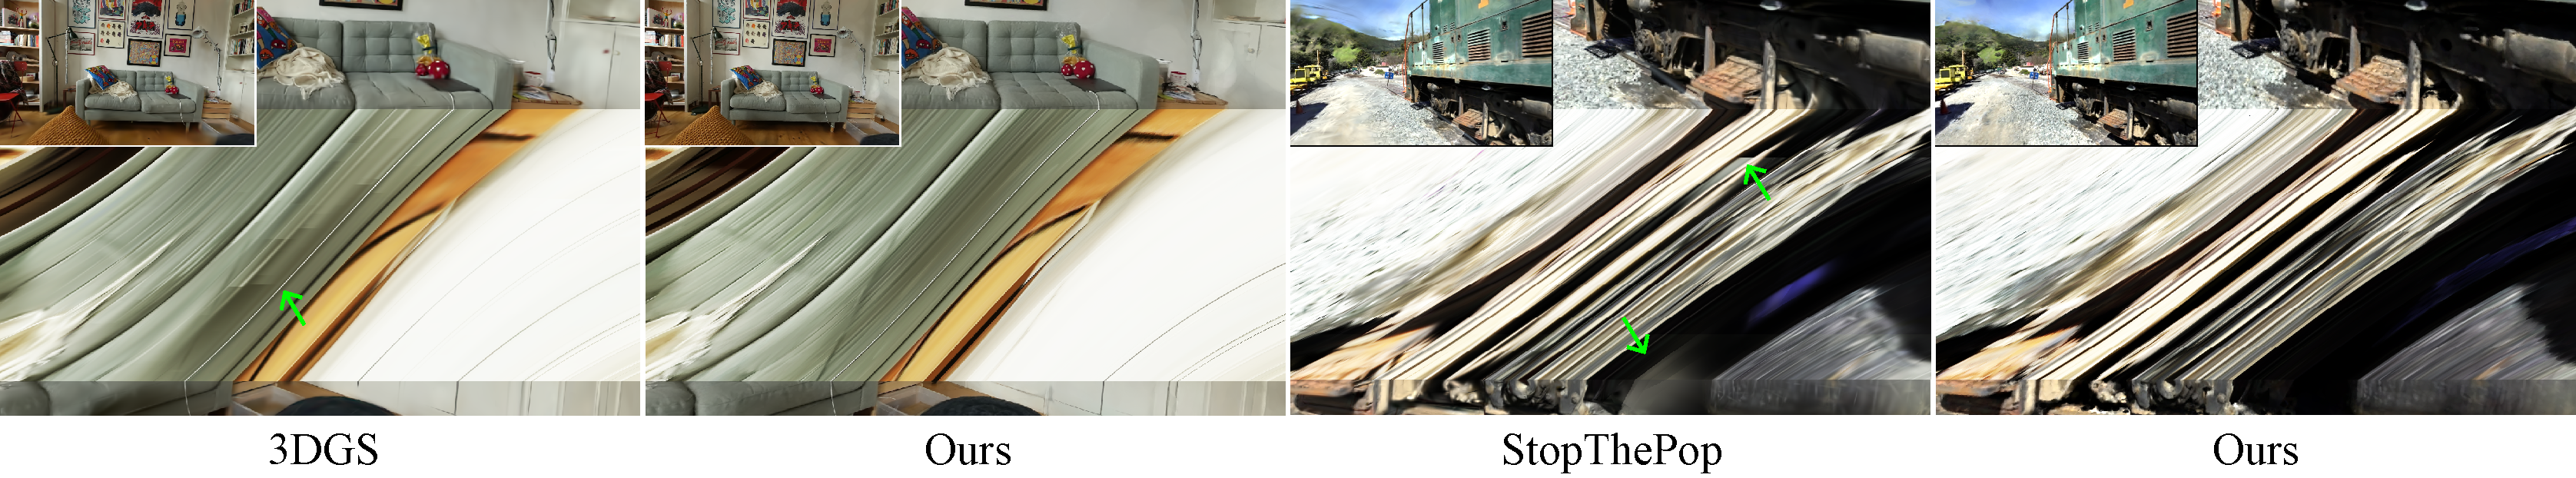
\includegraphics[width=\linewidth]{figures/EPIs_large_contrast.pdf}
\caption{
Here we show epipolar plane images \cite{bolles1987epipolar} to visualize popping in 3DGS~\cite{kerbl20233d} and StopThePop~\cite{radl2024stopthepop}. We recorded sequences of images while rotating the camera in the \scenename{berlin}~\cite{barron2023zip} (left) and \scenename{train}~\cite{knapitsch2017tanks} (right) scenes. The region in the middle are the epipolar plane images, with green arrows highlighting discontinuities in the color caused by popping/blend order artifacts. Our method lacks these horizontal discontinuities. Contrast and brightness have been boosted here for visibility's sake. See the supplemental video for more.}
\label{fig:popping_train}
\end{figure*}

\newcommand{\graphablation}[1]{
\begin{tikzpicture}[zoomboxarray]
    \node [image node] { \includegraphics[width=4.15cm]{#1} };
    \zoombox[magnification=6]{0.85,0.93}
    \zoombox[magnification=4]{0.6,0.55}
\end{tikzpicture}
}
% \begin{figure*}
%     \centering
%     \begin{tabular}{@{}cc@{}}
%     % \vspace{-3pt}
%     \graphablation{images/ablation/splatted.png} &
%     \graphablation{images/ablation/nomixing.png} \\
%     % \vspace{-3pt}
%     \small{(a) Splatted} & \small{(b) No Mixing} \\
%     \graphablation{images/ablation/ours.png} &
%     \graphablation{images/ablation/gt.png} \\
%     \small{(c) Volume Rendering (Ours)} & \small{(d) Ground Truth}
%     \end{tabular}
%     \vspace{-8pt}
%     \caption{To visualize the difference between rendering methods, we optimize our ellipsoids for our method, then visualize how different rendering methods affect the final image. Both ``Splatted'' and ``No Mixing'' assume that Gaussians do not overlap, with the former ordering them globally for the image (like 3DGS) , and the latter sorting them independently per pixel (like StopThePop). Both approaches cause hard edges to appear in areas where different primitives were blended to produce a color gradient.}
%     \label{fig:ablation}
% \end{figure*}


\subsection{Popping}

\begin{table}[b!]
\resizebox{\linewidth}{!}{
\large
\begin{tabular}{l|rr|rr|rr|rr}
StP Popping & \multicolumn{2}{l|}{DeepBlending}                                                      & \multicolumn{2}{l|}{M360 Indoor}                                                       & \multicolumn{2}{l|}{M360 Outdoor}                                                      & \multicolumn{2}{l}{Tanks \& Temples}                                                  \\
Metric      & \multicolumn{1}{l}{\reflectbox{F}LIP$_1$} & \multicolumn{1}{l|}{\reflectbox{F}LIP$_7$} & \multicolumn{1}{l}{\reflectbox{F}LIP$_1$} & \multicolumn{1}{l|}{\reflectbox{F}LIP$_7$} & \multicolumn{1}{l}{\reflectbox{F}LIP$_1$} & \multicolumn{1}{l|}{\reflectbox{F}LIP$_7$} & \multicolumn{1}{l}{\reflectbox{F}LIP$_1$} & \multicolumn{1}{l}{\reflectbox{F}LIP$_7$} \\ \hline
3DGS        & \cellcolor[HTML]{FFFFB4}0.0063            & \cellcolor[HTML]{FFFFB4}0.0122             & \cellcolor[HTML]{FFFFB4}0.0072            & \cellcolor[HTML]{FFFFB4}0.0149             & \cellcolor[HTML]{FFFFB4}0.0083            & \cellcolor[HTML]{FFFFB4}0.0154             & \cellcolor[HTML]{FFFFB4}0.0107            & \cellcolor[HTML]{FFFFB4}0.0315            \\
StopThePop  & \cellcolor[HTML]{FFD9B3}0.0052            & \cellcolor[HTML]{FFD9B3}0.0055             & \cellcolor[HTML]{FFD9B3}0.0060            & \cellcolor[HTML]{FFD9B3}0.0073             & \cellcolor[HTML]{FFD9B3}0.0083            & \cellcolor[HTML]{FFD9B3}0.0115             & \cellcolor[HTML]{FFD9B3}0.0076            & \cellcolor[HTML]{FFD9B3}0.0114            \\
Ours        & \cellcolor[HTML]{FFB3B3}0.0031            & \cellcolor[HTML]{FFB3B3}0.0000             & \cellcolor[HTML]{FFB3B3}0.0049            & \cellcolor[HTML]{FFB3B3}0.0000             & \cellcolor[HTML]{FFB3B3}0.0067            & \cellcolor[HTML]{FFB3B3}0.0000             & \cellcolor[HTML]{FFB3B3}0.0040            & \cellcolor[HTML]{FFB3B3}0.0000           
\end{tabular}
}\\
\caption{Experimental evidence that our method does not suffer popping, using the metric from StopThePop~\cite{radl2024stopthepop}. \reflectbox{F}LIP$_7$ is considered a more reliable step size by the authors because the signal is stronger than the noise caused by the optical flow used to compute the metric.}
\label{tab:popping}
\end{table}

As established in Figure~\ref{fig:popping_diagram}, both 3DGS and StopThePop exhibit artifacts due to their view-dependent density. We show what these artifacts look like using epipolar plane images \cite{bolles1987epipolar} in Figure~\ref{fig:popping_train}.
Because our rendering model is exact, and because the volume rendering integral is a continuous function of ray direction, our renderings exhibit no popping. Please see the supplemental video for a clear visualization.

To accompany our theoretical explanation of why our method does not suffer popping, we compare our method to StopThePop and 3DGS using the metric from StopThePop~(StP) to measure the amount of popping, closely following the original author's methodology across all the original scenes measured. EVER achieves a lower (better) score at step=1, and 0.0 error (lowest) with step=7, which StP called a more reliable step size, see Table.~\ref{tab:popping}. 

\subsection{Performance}
At 720p, we achieve average framerates of 36 FPS on the mip-NeRF 360 outdoor scenes, 66 FPS on the mip-NeRF 360 indoor scenes, and 30 FPS on the Zip-NeRF scenes on an NVIDIA RTX4090. The test set resolution is high on a couple of the Zip-NeRF and Mip-NeRF360 scenes, which causes the drop in FPS in Table~\ref{tab:main_results}. Training takes around 1-2 hours, also on an NVIDIA RTX4090. 
The majority of the time is spent tracing through the scene for rendering, which takes 20-71 ms, depending on the BVH.
For back propagation, 16 ms are spent storing intersections, and 13-20 ms are spent loading the primitives and atomically adding up the gradients. The BVH is rebuilt every training iteration, which takes 2-20 ms.

\newcommand{\graphimten}[1]{
\begin{tikzpicture}[zoomboxarray, zoomboxarray rows=1, zoomboxes below, zoomboxarray inner gap=0.0cm]
    \node [image node] { \includegraphics[width=4.5cm,valign=b]{#1} };
    \zoombox[magnification=4]{0.125,0.54}
\end{tikzpicture}
}

\begin{table}[b!]
\resizebox{\linewidth}{!}{
\large
\begin{tabular}{l|ccc|c}
                   & \multicolumn{1}{c}{PSNR$\uparrow$} & \multicolumn{1}{c}{SSIM$\uparrow$} & \multicolumn{1}{c|}{LPIPS$\downarrow$} & \multicolumn{1}{c}{FPS$\uparrow$}               \\ \hline
Splatted           & 26.63                               & .845                                & .329                                    & -                                                \\
No Mixing          & 26.79                               & .849                                & .305                                    & -                                                \\
3DGS               & 27.02                               & .853                                & .301                                    & -                                                \\
3DGS + Our Changes & 26.94                               & .832                                & .323                                    & -                                                \\
No Anisotropic     & \cellcolor[HTML]{FFB3B3}27.25       & \cellcolor[HTML]{FFB3B3}.865        & \cellcolor[HTML]{FFB3B3}.272            & \multicolumn{1}{r}{27.3}                         \\
No Points          & \cellcolor[HTML]{FFD9B3}27.19       & \cellcolor[HTML]{FFD9B3}.863        & \cellcolor[HTML]{FFD9B3}.277            & \multicolumn{1}{r}{\cellcolor[HTML]{FFFFB4}41.2} \\
No Rand Center     & 27.08                               & .859                                & \cellcolor[HTML]{FFFFB4}.278            & \multicolumn{1}{r}{\cellcolor[HTML]{FFD9B3}41.4} \\ \hline
Ours               & \cellcolor[HTML]{FFFFB4}27.17       & \cellcolor[HTML]{FFFFB4}.862        & \cellcolor[HTML]{FFD9B3}.277            & \multicolumn{1}{r}{\cellcolor[HTML]{FFB3B3}41.9}
\end{tabular}
}\\
\caption{
An ablation study reporting average performance on the \scenename{bicycle} and \scenename{counter} scenes from MipNeRF 360~\cite{barron2021mip} and the \scenename{berlin} scene from ZipNeRF~\cite{barron2023zip}. The ``No Anisotropic'' ablation shows the cost of our regularizer that increases frame-rate.}
\label{tab:ablation}
\end{table}

\subsection{Ablations}
To see if it was possible to train our model using ray tracing, then render using splatting, we implemented a splatting version of our 3D ellipsoids, labeled ``Splatted''. We also tested what would happen if we sorted the primitives per ray like StopThePop without our color blending technique, which is labeled ``No Mixing''. Both of these resulted in visual degradation in areas where the method had been mixing primitive colors together, which can be seen on the fridge and candle. 
These ablations also perform worse when trained for their specific rendering styles, as can be seen in Table~\ref{tab:ablation}. ``Splatting'' performs worse than ``No Mixing'', which does not match the comparison between 3DGS and StopThePop, both of which have similar performance. %This could be an indication that per ray sorting provides some kind of improved blending.

To ablate the effect of our densification changes, along with the other changes, we use the 3DGS renderer with the other minor changes we've made to densification, which we label ``3DGS + Our Changes''.
These changes do not help 3DGS because they are aimed at handling density primitives. 
Finally, we run ablations on each of the changes we performed.
``No anisotropic'' refers to ablating anisotropic loss, which results in slightly increased quality, but much lower framerate. ``No points'' refers to no additional points added using the inverse contraction, which reduces the reliance on the SfM reconstruction. The inverse contraction sampling is described in the supplemental material.
%, which has almost no effect on the quality, but is useful on datasets where the SfM wasn't very good, like London.
``No Rand Centers'' refers to ablating randomizing the pixel centers, which helps with thin structures on the bicycle scene.
We jitter our rays by picking a point within the pixel from a uniform random distribution, as opposed to using the center of the pixel. 

\section{Conclusion}

% Order of claims: 
% 1. We introduce exact volume rendering for infinite overlapping primitives in real time
% 2. We observe that this improves smooth textures on walls
% 3. This results in better performance on larger scenes
% 4. This is possible with our double intersection approach
% 5. Which we combine with ray tracing for flexible rendering
% Higher than ZipNeRF with SSIM and matching on LPIPS

% We find that our method outperforms Zip-NeRF on the larger Zip-NeRF datasets on sharpness, while outperforming all other real-time methods on SSIM and LPIPS on the Mip-NeRF360 and Zip-NeRF datasets.
% By isolating the effect of our renderer, we know that this improvement comes from a combination of density based primitives and double-intersection based perfect blending.
% 

Our double-intersection approach for \longname{} can be used to blend any number of overlapping primitive colors in a physically accurate way. We have shown that our method outperforms Zip-NeRF on the larger Zip-NeRF datasets on sharpness, while outperforming all other real-time methods on SSIM and LPIPS on the Mip-NeRF360 and Zip-NeRF datasets. By isolating the effect of our renderer, we know that this improvement comes from a combination of density based primitives and double-intersection based, physically accurate blending.
This results in an approach that bridges the gap between slow but accurate radiance field methods such as Zip-NeRF, and fast but inaccurate radiance field methods like 3DGS. 

We also show that sorting primitives per a pixel is not sufficient for eliminating the popping artifacts in 3DGS. It is only by combining per pixel sorting, which we achieve with ray tracing, with proper primitive blending, that we are able to eliminate these artifacts. %Our use of ray-tracing also enables lens blur and fisheye camera distortion
Together, \acronym{} is able to produce high-quality, large scale renderings that are guaranteed to be 3D-consistent, and does so at 30 FPS at 720p on a single NVIDIA RTX4090. 
% \acronym{} enables highly-flexible, high-quality, real-time, large scale, radiance field reconstruction.

% By combining the flexibility of ray-tracing with the speed of primitive-based radiance field methods, 


%We have presented \longname{} (\acronym{}), which bridges the gap between slow but accurate radiance field methods such as Zip-NeRF, and fast but inaccurate radiance field methods like 3DGS.Our method is capable of handling exact volume rendering for infinite overlapping primitives in real time, enabling smooth textures on walls and better performance on larger scenes. This is achieved through our double intersection method, combined with ray tracing for flexible, high-quality rendering.
%By exactly ray-tracing a volumetric collection of constant density ellipsoids, \acronym{} is able to produce high-quality renderings that are guaranteed to be 3D-consistent and therefore exhibit no popping, and does so at 30 FPS at 720p on a single NVIDIA RTX4090. By combining the flexibility of ray-tracing with the speed of primitive-based radiance field methods, \acronym{} enables highly-flexible, high-quality, real-time, radiance field reconstruction.


\iftoggle{cvprfinal}{
\myparagraph{Acknowledgements}
We would like to thank Delio Vicini, Stephan Garbin and Ben Lee for helpful discussions.
AM is funded in part by the USACE Engineer Research and Development Center Cooperative Agreement W9132T-22-2-0014.
}{}


{
    \small
    \bibliographystyle{ieeenat_fullname}
    \bibliography{main}
}

% WARNING: do not forget to delete the supplementary pages from your submission 
\iftoggle{cvprfinal}{
\appendix
\clearpage
\setcounter{page}{1}
\maketitlesupplementary


\section{Backpropagation}
We use an adjoint rendering approach, starting from the last state of each ray, which we store, and reconstruct each ray state backwards using $p^{-1}(x, i)$. We can then use this reconstructed state to backpropagate the error to each state, then propagate this error to each primitive. The gradient with respect to mean, scale, and orientation, all come from the derivative of the ray-ellipsoid intersection function.  
To retrieve the list of primitives intersected, we store the list of intersections on the forward pass. Since rays tend to terminate before 300 total intersections, this turns out to be relatively cheap, at 1.2 KB per a ray. Although we experimented with using ray tracing to retrieve the list of surfaces in reverse order, we found the instability too high. 


\begin{figure*}[ht]
\centering
\bgroup
% \def\arraystretch{2}
\begin{tabular}{@{}c@{}c@{}c@{}c@{}c@{}}
\graphimtwelve{images/comparison_table_jpg/3DGS_im12.jpg} &
% \graphimtwelve{images/comparison_table_jpg/mcmc_im12.jpg} &
\graphimtwelve{images/comparison_table_jpg/stop_im12.jpg} &
% \graphimtwelve{images/comparison_table_jpg/3dgrt_im12.jpg} &
\graphimtwelve{images/comparison_table_jpg/smerf_im12.jpg} &
\graphimtwelve{images/comparison_table_jpg/ours_im12.jpg} &
\graphimtwelve{images/comparison_table_jpg/gt_im12.jpg} \\
% \raisebox{3.0cm}{\textbf{(b)}} &
\graphimthirteen{images/comparison_table_jpg/3DGS_im13.jpg} &
% \graphimthirteen{images/comparison_table_jpg/mcmc_im13.jpg} &
\graphimthirteen{images/comparison_table_jpg/stop_im13.jpg} &
% \graphimthirteen{images/comparison_table_jpg/3dgrt_im13.jpg} &
\graphimthirteen{images/comparison_table_jpg/smerf_im13.jpg} &
\graphimthirteen{images/comparison_table_jpg/ours_im13.jpg} &
\graphimthirteen{images/comparison_table_jpg/gt_im13.jpg} \\
% \graphimone{images/comparison_table_jpg/3DGS_im1.jpg} &
% \graphimone{images/comparison_table_jpg/mcmc_im1.jpg} &
% \graphimone{images/comparison_table_jpg/stop_im1.jpg} &
% \graphimone{images/comparison_table_jpg/ours_im1.jpg} &
% \graphimone{images/comparison_table_jpg/gt_im1.jpg} \\
\graphimseven{images/comparison_table_jpg/3DGS_im7.jpg} &
% \graphimseven{images/comparison_table_jpg/mcmc_im7.jpg} &
\graphimseven{images/comparison_table_jpg/stop_im7.jpg} &
% \graphimseven{images/comparison_table_jpg/3dgrt_im7.jpg} &
\graphimseven{images/comparison_table_jpg/smerf_im7.jpg} &
\graphimseven{images/comparison_table_jpg/ours_im7.jpg} &
\graphimseven{images/comparison_table_jpg/gt_im7.jpg} \\

\graphimfourteen{images/comparison_table_jpg/3DGS_im14.jpg} &
% \graphimfourteen{images/comparison_table_jpg/mcmc_im14.jpg} &
\graphimfourteen{images/comparison_table_jpg/stop_im14.jpg} &
% \graphimfourteen{images/comparison_table_jpg/3dgrt_im14.jpg} &
\graphimfourteen{images/comparison_table_jpg/smerf_im14.jpg} &
\graphimfourteen{images/comparison_table_jpg/ours_im14.jpg} &
\graphimfourteen{images/comparison_table_jpg/gt_im14.jpg} \\
% \graphimeleven{images/comparison_table_jpg/3DGS_im11.jpg} &
% \graphimeleven{images/comparison_table_jpg/mcmc_im11.jpg} &
% \graphimeleven{images/comparison_table_jpg/stop_im11.jpg} &
% \graphimeleven{images/comparison_table_jpg/ours_im11.jpg} &
% \graphimeleven{images/comparison_table_jpg/gt_im11.jpg} \\

% \graphimtwo{images/comparison_table_jpg/3DGS_im2.jpg} &
% \graphimtwo{images/comparison_table_jpg/mcmc_im2.jpg} &
% \graphimtwo{images/comparison_table_jpg/stop_im2.jpg} &
% \graphimtwo{images/comparison_table_jpg/ours_im2.jpg} &
% \graphimtwo{images/comparison_table_jpg/gt_im2.jpg} \\

% \graphimnine{images/comparison_table_jpg/3DGS_im9.jpg} &
% % \graphimnine{images/comparison_table_jpg/mcmc_im9.jpg} &
% \graphimnine{images/comparison_table_jpg/stop_im9.jpg} &
% \graphimnine{images/comparison_table_jpg/ours_im9.jpg} &
% \graphimnine{images/comparison_table_jpg/gt_im9.jpg} \\
3DGS & StopThePop & SMERF & Ours & GT
\end{tabular}
\egroup
\caption{Additional visual comparison of our method on the Mip-NeRF 360 dataset~\cite{barron2023zip}.}
\label{fig:comparison_supp}
\end{figure*}

\begin{table*}[ht]
    \centering
    \begin{tabular}{l|rrrrr}
\rowcolor[HTML]{F1F3F4} 
\textbf{PSNR $\uparrow$}    & \multicolumn{1}{l}{\cellcolor[HTML]{F1F3F4}berlin} & \multicolumn{1}{l}{\cellcolor[HTML]{F1F3F4}nyc} & \multicolumn{1}{l}{\cellcolor[HTML]{F1F3F4}alameda} & \multicolumn{1}{l}{\cellcolor[HTML]{F1F3F4}london} & \multicolumn{1}{l}{\cellcolor[HTML]{F1F3F4}Average} \\ \hline
3DGS                        & \cellcolor[HTML]{FFFFB4}26.83                      & 26.90                                           & \cellcolor[HTML]{FFFFB4}24.14                       & 25.48                                              & 25.84                                               \\
Mip Splatting               & \cellcolor[HTML]{FFB3B3}27.30                      & \cellcolor[HTML]{FFD9B3}27.52                   & \cellcolor[HTML]{FFB3B3}24.76                       & \cellcolor[HTML]{FFD9B3}26.28                      & \cellcolor[HTML]{FFD9B3}26.46                       \\
StopThePop                  & 26.81                                              & \cellcolor[HTML]{FFFFB4}27.14                   & 24.12                                               & \cellcolor[HTML]{FFFFB4}25.61                      & \cellcolor[HTML]{FFFFB4}25.92                       \\
SMERF                       & 28.52                                              & \cellcolor[HTML]{FFFFB4}28.21                   & 25.35                                               & \cellcolor[HTML]{FFFFB4}27.05                      & \cellcolor[HTML]{FFFFB4}27.28                       \\
Ours                        & 27.24                                              & 27.93                                           & 24.72                                               & 26.49                                              & \cellcolor[HTML]{FFB3B3}26.60                       \\ \hline
Zip-NeRF                    & 28.59                                              & 28.42                                           & 25.41                                               & 27.06                                              & 27.37                                               \\ \hline
\rowcolor[HTML]{F1F3F4} 
\textbf{SSIM $\uparrow$}    & \multicolumn{1}{l}{\cellcolor[HTML]{F1F3F4}berlin} & \multicolumn{1}{l}{\cellcolor[HTML]{F1F3F4}nyc} & \multicolumn{1}{l}{\cellcolor[HTML]{F1F3F4}alameda} & \multicolumn{1}{l}{\cellcolor[HTML]{F1F3F4}london} & \multicolumn{1}{l}{\cellcolor[HTML]{F1F3F4}Average} \\ \hline
3DGS                        & .899                                               & .861                                            & .776                                                & .830                                               & .842                                                \\
Mip Splatting               & \cellcolor[HTML]{FFD9B3}.892                       & \cellcolor[HTML]{FFD9B3}.853                    & \cellcolor[HTML]{FFD9B3}.768                        & \cellcolor[HTML]{FFD9B3}.822                       & \cellcolor[HTML]{FFD9B3}.834                        \\
StopThePop                  & \cellcolor[HTML]{FFFFB4}.885                       & \cellcolor[HTML]{FFFFB4}.844                    & \cellcolor[HTML]{FFFFB4}.748                        & \cellcolor[HTML]{FFFFB4}.801                       & \cellcolor[HTML]{FFFFB4}.819                        \\
SMERF                       & \cellcolor[HTML]{FFFFB4}.887                       & \cellcolor[HTML]{FFFFB4}.844                    & \cellcolor[HTML]{FFFFB4}.758                        & \cellcolor[HTML]{FFFFB4}.829                       & \cellcolor[HTML]{FFFFB4}.830                        \\
Ours                        & \cellcolor[HTML]{FFB3B3}.900                       & \cellcolor[HTML]{FFB3B3}.863                    & \cellcolor[HTML]{FFB3B3}.779                        & \cellcolor[HTML]{FFB3B3}.837                       & \cellcolor[HTML]{FFB3B3}.845                        \\ \hline
Zip-NeRF                    & .891                                               & .850                                            & .767                                                & .835                                               & .836                                                \\ \hline
\rowcolor[HTML]{F1F3F4} 
\textbf{LPIPS $\downarrow$} & \multicolumn{1}{l}{\cellcolor[HTML]{F1F3F4}berlin} & \multicolumn{1}{l}{\cellcolor[HTML]{F1F3F4}nyc} & \multicolumn{1}{l}{\cellcolor[HTML]{F1F3F4}alameda} & \multicolumn{1}{l}{\cellcolor[HTML]{F1F3F4}london} & \multicolumn{1}{l}{\cellcolor[HTML]{F1F3F4}Average} \\ \hline
3DGS                        & \cellcolor[HTML]{FFFFB4}.406                       & \cellcolor[HTML]{FFFFB4}.380                    & \cellcolor[HTML]{FFFFB4}.441                        & \cellcolor[HTML]{FFFFB4}.446                       & \cellcolor[HTML]{FFFFB4}.418                        \\
Mip Splatting               & .392                                               & .356                                            & .410                                                & .411                                               & .392                                                \\
StopThePop                  & \cellcolor[HTML]{FFD9B3}.402                       & \cellcolor[HTML]{FFD9B3}.373                    & \cellcolor[HTML]{FFD9B3}.433                        & \cellcolor[HTML]{FFD9B3}.438                       & \cellcolor[HTML]{FFD9B3}.411                        \\
SMERF                       & \cellcolor[HTML]{FFD9B3}.391                       & \cellcolor[HTML]{FFD9B3}.361                    & \cellcolor[HTML]{FFD9B3}.416                        & \cellcolor[HTML]{FFD9B3}.390                       & \cellcolor[HTML]{FFD9B3}.389                        \\
Ours                        & \cellcolor[HTML]{FFB3B3}.371                       & \cellcolor[HTML]{FFB3B3}.337                    & \cellcolor[HTML]{FFB3B3}.389                        & \cellcolor[HTML]{FFB3B3}.374                       & \cellcolor[HTML]{FFB3B3}.368                        \\ \hline
Zip-NeRF                    & .378                                               & .331                                            & .387                                                & .360                                               & .364                                               
\end{tabular}
    \caption{Full results for Zip-NeRF dataset}
    % \label{tab:full_zipnerf}
    \centering
    \begin{tabular}{l|rrrrr|rrrr}
\rowcolor[HTML]{F1F3F4} 
\textbf{PSNR $\uparrow$}    & \multicolumn{1}{l}{\cellcolor[HTML]{F1F3F4}bicycle} & \multicolumn{1}{l}{\cellcolor[HTML]{F1F3F4}flowers} & \multicolumn{1}{l}{\cellcolor[HTML]{F1F3F4}garden} & \multicolumn{1}{l}{\cellcolor[HTML]{F1F3F4}stump} & \multicolumn{1}{l|}{\cellcolor[HTML]{F1F3F4}treehill} & \multicolumn{1}{l}{\cellcolor[HTML]{F1F3F4}room} & \multicolumn{1}{l}{\cellcolor[HTML]{F1F3F4}counter} & \multicolumn{1}{l}{\cellcolor[HTML]{F1F3F4}kitchen} & \multicolumn{1}{l}{\cellcolor[HTML]{F1F3F4}bonsai} \\ \hline
3DGS                        & \cellcolor[HTML]{FFFFB4}25.24                       & 21.55                                               & \cellcolor[HTML]{FFFFB4}27.38                      & 26.56                                             & 22.43                                                 & \cellcolor[HTML]{FFD9B3}31.53                    & \cellcolor[HTML]{FFFFB4}29.00                       & \cellcolor[HTML]{FFD9B3}31.45                       & \cellcolor[HTML]{FFFFB4}32.21                      \\
StopThePop                  & 25.23                                               & \cellcolor[HTML]{FFFFB4}21.62                       & 27.33                                              & \cellcolor[HTML]{FFD9B3}26.65                     & \cellcolor[HTML]{FFFFB4}22.44                         & 30.91                                            & 28.79                                               & \cellcolor[HTML]{FFFFB4}31.13                       & 31.85                                              \\
3DGRT                       & 25.13                                               & 21.58                                               & 26.99                                              & \cellcolor[HTML]{FFFFB4}26.57                     & 22.40                                                 & 30.92                                            & 28.78                                               & 30.60                                               & 31.85                                              \\
SMERF                       & \cellcolor[HTML]{FFB3B3}25.58                       & \cellcolor[HTML]{FFB3B3}22.24                       & \cellcolor[HTML]{FFB3B3}27.66                      & \cellcolor[HTML]{FFB3B3}27.19                     & \cellcolor[HTML]{FFB3B3}23.93                         & \cellcolor[HTML]{FFFFB4}31.38                    & \cellcolor[HTML]{FFB3B3}29.02                       & \cellcolor[HTML]{FFB3B3}31.68                       & \cellcolor[HTML]{FFB3B3}33.19                      \\
Our model                   & \cellcolor[HTML]{FFD9B3}25.34                       & \cellcolor[HTML]{FFD9B3}21.70                       & \cellcolor[HTML]{FFD9B3}27.46                      & 26.41                                             & \cellcolor[HTML]{FFD9B3}22.74                         & \cellcolor[HTML]{FFB3B3}31.39                    & \cellcolor[HTML]{FFD9B3}28.91                       & 31.36                                               & \cellcolor[HTML]{FFD9B3}32.24                      \\ \hline
ZipNeRF                     & 25.80                                               & 22.40                                               & 28.20                                              & 27.55                                             & 23.89                                                 & 32.65                                            & 29.38                                               & 32.50                                               & 34.46                                              \\ \hline
\rowcolor[HTML]{F1F3F4} 
\textbf{SSIM $\uparrow$}    & \multicolumn{1}{l}{\cellcolor[HTML]{F1F3F4}bicycle} & \multicolumn{1}{l}{\cellcolor[HTML]{F1F3F4}flowers} & \multicolumn{1}{l}{\cellcolor[HTML]{F1F3F4}garden} & \multicolumn{1}{l}{\cellcolor[HTML]{F1F3F4}stump} & \multicolumn{1}{l|}{\cellcolor[HTML]{F1F3F4}treehill} & \multicolumn{1}{l}{\cellcolor[HTML]{F1F3F4}room} & \multicolumn{1}{l}{\cellcolor[HTML]{F1F3F4}counter} & \multicolumn{1}{l}{\cellcolor[HTML]{F1F3F4}kitchen} & \multicolumn{1}{l}{\cellcolor[HTML]{F1F3F4}bonsai} \\ \hline
3DGS                        & .766                                                & .606                                                & \cellcolor[HTML]{FFD9B3}.866                       & .771                                              & .633                                                  & \cellcolor[HTML]{FFD9B3}.919                     & \cellcolor[HTML]{FFD9B3}.909                        & \cellcolor[HTML]{FFB3B3}.928                        & \cellcolor[HTML]{FFB3B3}.942                       \\
StopThePop                  & \cellcolor[HTML]{FFFFB4}.768                        & .607                                                & \cellcolor[HTML]{FFD9B3}.866                       & .775                                              & .635                                                  & \cellcolor[HTML]{FFD9B3}.919                     & .907                                                & \cellcolor[HTML]{FFD9B3}.927                        & \cellcolor[HTML]{FFFFB4}.941                       \\
3DGRT                       & \cellcolor[HTML]{FFD9B3}.770                        & \cellcolor[HTML]{FFFFB4}.624                        & \cellcolor[HTML]{FFFFB4}.858                       & \cellcolor[HTML]{FFFFB4}.779                      & \cellcolor[HTML]{FFFFB4}.636                          & .917                                             & \cellcolor[HTML]{FFFFB4}.908                        & .924                                                & \cellcolor[HTML]{FFB3B3}.942                       \\
SMERF                       & .760                                                & \cellcolor[HTML]{FFD9B3}.626                        & .844                                               & \cellcolor[HTML]{FFB3B3}.784                      & \cellcolor[HTML]{FFB3B3}.682                          & \cellcolor[HTML]{FFFFB4}.918                     & .892                                                & .916                                                & \cellcolor[HTML]{FFFFB4}.941                       \\
Our model                   & \cellcolor[HTML]{FFB3B3}.776                        & \cellcolor[HTML]{FFB3B3}.639                        & \cellcolor[HTML]{FFB3B3}.869                       & \cellcolor[HTML]{FFD9B3}.781                      & \cellcolor[HTML]{FFD9B3}.656                          & \cellcolor[HTML]{FFB3B3}.922                     & \cellcolor[HTML]{FFB3B3}.910                        & \cellcolor[HTML]{FFFFB4}.926                        & \cellcolor[HTML]{FFD9B3}.943                       \\ \hline
ZipNeRF                     & .769                                                & .642                                                & .860                                               & .800                                              & .681                                                  & .925                                             & .902                                                & .928                                                & .949                                               \\ \hline
\rowcolor[HTML]{F1F3F4} 
\textbf{LPIPS $\downarrow$} & \multicolumn{1}{l}{\cellcolor[HTML]{F1F3F4}bicycle} & \multicolumn{1}{l}{\cellcolor[HTML]{F1F3F4}flowers} & \multicolumn{1}{l}{\cellcolor[HTML]{F1F3F4}garden} & \multicolumn{1}{l}{\cellcolor[HTML]{F1F3F4}stump} & \multicolumn{1}{l|}{\cellcolor[HTML]{F1F3F4}treehill} & \multicolumn{1}{l}{\cellcolor[HTML]{F1F3F4}room} & \multicolumn{1}{l}{\cellcolor[HTML]{F1F3F4}counter} & \multicolumn{1}{l}{\cellcolor[HTML]{F1F3F4}kitchen} & \multicolumn{1}{l}{\cellcolor[HTML]{F1F3F4}bonsai} \\ \hline
3DGS                        & .240                                                & .367                                                & \cellcolor[HTML]{FFD9B3}.123                       & .251                                              & .376                                                  & .287                                             & .258                                                & \cellcolor[HTML]{FFD9B3}.155                        & .252                                               \\
StopThePop                  & \cellcolor[HTML]{FFFFB4}.233                        & .362                                                & \cellcolor[HTML]{FFB3B3}.120                       & \cellcolor[HTML]{FFFFB4}.244                      & .366                                                  & .281                                             & \cellcolor[HTML]{FFFFB4}.253                        & \cellcolor[HTML]{FFB3B3}.154                        & .249                                               \\
3DGRT                       & \cellcolor[HTML]{FFD9B3}.226                        & \cellcolor[HTML]{FFFFB4}.335                        & \cellcolor[HTML]{FFFFB4}.134                       & \cellcolor[HTML]{FFD9B3}.243                      & \cellcolor[HTML]{FFFFB4}.364                          & \cellcolor[HTML]{FFFFB4}.280                     & \cellcolor[HTML]{FFD9B3}.248                        & \cellcolor[HTML]{FFFFB4}.156                        & \cellcolor[HTML]{FFFFB4}.242                       \\
SMERF                       & .239                                                & \cellcolor[HTML]{FFD9B3}.317                        & .147                                               & \cellcolor[HTML]{FFD9B3}.243                      & \cellcolor[HTML]{FFB3B3}.302                          & \cellcolor[HTML]{FFB3B3}.259                     & .256                                                & \cellcolor[HTML]{FFD9B3}.155                        & \cellcolor[HTML]{FFB3B3}.222                       \\
Our model                   & \cellcolor[HTML]{FFB3B3}.220                        & \cellcolor[HTML]{FFB3B3}.307                        & \cellcolor[HTML]{FFB3B3}.120                       & \cellcolor[HTML]{FFB3B3}.230                      & \cellcolor[HTML]{FFD9B3}.318                          & \cellcolor[HTML]{FFD9B3}.275                     & \cellcolor[HTML]{FFB3B3}.240                        & \cellcolor[HTML]{FFD9B3}.155                        & \cellcolor[HTML]{FFD9B3}.236                       \\ \hline
ZipNeRF                     & .228                                                & .309                                                & .127                                               & .236                                              & .281                                                  & .238                                             & .223                                                & .134                                                & .196                                              
\end{tabular}
    \caption{Full results for Mip-NeRF 360 dataset}
    \label{tab:full_mipnerf}
\end{table*}

\section{Hyperparameters, Etc} \label{sec:hparams}
We change the opacity learning rate to $0.0125$, the initial position learning rate to $4\times10^{-5}$ and the final position learning rate to $4\times10^{-7}$. We change the parameter known as ``percent dense'' in 3DGS to $0.001785$, which controls the size threshold above which primitives are split instead of cloned. We perform this every 200 iterations, instead of 100, and set the splitting gradient threshold to $2.5\times10^{-7}$ and the clone gradient threshold to $0.1$. We also stop splitting and cloning at 7 million primitives, or at 16000 iterations, which ever comes first, and start at 1500 iterations.

For color, we apply a softplus activation ($\beta=10$) to the output of the spherical harmonics (instead of 3DGS's relu activation), which we find avoids certain local minima where primitives get locked into a color. We increase the spherical harmonic degree every $2,\!000$ iterations, instead of $1,\!000$. We set the max primitive size to $25$ units, which improves performance.


\subsection{Inverse Contraction Initialization}
To help initialize the primitives in a scene, we supplement the SfM initialization with $10,\!000$ additional primitives. We generate these primitives by sampling their means uniformly from a radius-2 sphere. The radius is set to a constant value based the max radius at which the spheres could be packed into the radius-2 sphere, and colors are set to a constant value of $0.5$.
These primitives are then transformed by ``uncontracting'' the resulting means and covariances using the inverse of the contraction used in mip-NeRF 360~\cite{barron2022mip}. We found that highly anisotropic primitives at initialization can cause issues, so we scale the primitives to be isotropic.

To review, the mip-NeRF 360 contraction function $\mathcal{C}$ that maps from a 3D coordinate in Euclidean space $\mathbf{x}$ to a 3D coordinate in contracted space $\mathbf{z}$ is:
\begin{equation}
  \mathcal{C}(\mathbf{x}) = \mathbf{x} \cdot \frac{2 \sqrt{\max(1, || \mathbf{x} ||^2)} - 1}{\max(1, || \mathbf{x} ||^2)}
\end{equation}
The inverse of $\mathcal{C}(\mathbf{x})$ can be defined straightforwardly:
\begin{equation}
    \mathcal{C}^{-1}(\mathbf{z}) = \frac{\mathbf{z}}{\sqrt{\max(1, ||\mathbf{z}||^2)} (2 - \min(2, \sqrt{\max(1, ||\mathbf{z}||^2)}))}
\end{equation}
To apply this inverse contraction to a Gaussian instead of a point, we use the same Kalman-esque approach as was used in mip-NeRF 360: we linearize the contraction around $\mathbf{z}$ into a Jacobian-vector product, which we apply twice to the input covariance matrix.

}{}
\appendix

\end{document}
